\documentclass[11pt,a4paper]{article}

\usepackage[margin=1in, paperwidth=8.3in, paperheight=11.7in]{geometry}
\usepackage{amsmath,amsfonts,fancyhdr,graphicx,caption,subcaption}
\graphicspath{ {img/} }
\usepackage[section,nohyphen]{DomH}
\headertitle{Internet Economics and Financial Technology - Notes}

\begin{document}

\title{Internet Economics and Financial Technology - Notes}
\author{Dom Hutchinson}
\date{\today}
\maketitle

\tableofcontents\newpage

\section{The Big Picture}

  \begin{remark}{History of Commercial Computing}
    \begin{itemize}
      \item[\textit{1950-60}] Mainframes - slow; size of rooms.
      \item[\textit{1960-70}] Minicomputers - slow; couple per rooms.
      \item[\textit{1970-80}] PCs - faster; one per desk.
      \item[\textit{1980-90}] LANs - distributed networks.
      \item[\textit{1990-10}] Internet - world wide distributed network.
      \item[\textit{2010-20}] Cloud Computing
    \end{itemize}
    Where does IT go next? Has it peaked as IT is almost fully diffused?
  \end{remark}

  \begin{remark}{Economics in Computer Science}
    \textit{Market Economics} is a useful metaphor for new methods in computer science \& engineering which deal with allocation of scare resources. This is field is known as \textit{Market Based Control}. Algorithms in this field tend to model sellers \& buyers, and are applicable across most problems in the field (from server allocation to automated stock traders).
  \end{remark}

\section{Economic Principles}

  \begin{definition}{Externality}
    The production or consumption of a good has an \textit{externality} if it affects a third party who was not involved in the transaction. e.g. Pollution from production is a negative externality; education is a positive externality.
  \end{definition}

\subsection{Micro-Economics}

  \begin{definition}{Microeconomics}
    The study of the behaviour of \underline{individual economic actors} (individuals \& business) and how decisions are made based on the allocation of limited resources.
  \end{definition}

  \begin{definition}{Production-Consumption Cycle}
    Producers produce goods \& services which consumers wish to buy. Consumers have a limited about of money so have to choose what to \& to-not buy at given prices. Similarly, producers have a limited number of resources (raw, labour \& capital) so need to decide what goods \& services, at what price, to produce. These lead to the idea of supply \& demand curves.
  \end{definition}

  \begin{definition}{Supply and Demand Equilibrium}
    The \textit{Equilibrium} of a supply-and-demand curve is a \textit{price} where the quantity demanded by all consumers is \underline{equal to} the quantity supplied by all producers.
    \par When there is \textit{excess demand} prices will rise due to scarcity of supply. The increase in supply will reduce demand as some consumers will not be happy to pay the higher price, meaning a new (higher) \textit{equilibrium price} will be reached.
    \par If there is \textit{excess supply} prices will decrease as producers try to encourage customers to buy their product over others, this will in turn attract new customers and cause some producers out of business. A new lower \textit{equilibrium price} will be reached.
  \end{definition}

  \begin{definition}{Consumer Demand Curve}
    A consumer's \textit{Demand Curve} plots the quantity of a product a consumer is willing to buy for a given price-per-unit. These are typically downwards sloping as consumers prefer to pay lower prices. It is assumed a consumer will buy the quantity of units equal to the point where the \textit{Demand Curve} intersects the market price.

    \par The area under the curve, but above the \textit{Market Price} is known as \textit{Consumer Surplus}. This quantifies how much more a given consumer was willing to pay than the market price. The number of items a consumer is willing to buy at the \textit{Market Price} \underline{multiplied} by the \textit{Market Price} gives the \textit{Expenditure} for that consumer. Consumers want to maximise \textit{Consumer Surplus}.

    \par See \texttt{Figure 2}
  \end{definition}

  \begin{figure}[ht!]
    \centering
    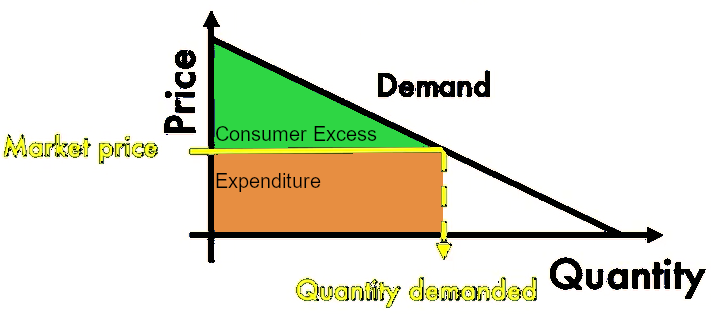
\includegraphics[width=.5\textwidth]{consumerSurplus.PNG}
    \caption{Consumer Surplus \& Expenditure}
  \end{figure}

  \begin{definition}{Production Costs}
    A producer will have costs they need to pay in order to stay in business. These costs can be categorised as
    \begin{itemize}
      \item[\textit{Fixed Costs}] A company must incur in order to operate, even before they start producing. (e.g. rent)
      \item[\textit{Variable Costs}] are costs which depend on the number of units produced. (e.g. equipment, raw materials)
      \item[\textit{Semi-Variable Costs}] Labour can be considered a variable cost as you can choose to pay overtime or to hire someone new in order to increase production.
    \end{itemize}
    The sum of these values will give you the \textit{Total Cost} of production.
  \end{definition}

  \begin{definition}{Marginal Cost Curve}
    \textit{Marginal Cost} is the cost of producing the \underline{last} unit. It is equal to
    \[ \dfrac{\text{Change in Cost}}{\text{Change in Quantity Produced}} \]
    \par We can plot a \textit{Marginal Cost Curve} of marginal cost against quantity. Typically these are initially downwards sloping, then upwards sloping.
  \end{definition}

  \begin{definition}{Economies of Scale}
    When the \textit{Marginal Cost Curve} is downwards sloping \textit{Economies of Scale} are being experienced. \textit{Economies of Scale} are the cost advantages a producer obtains by scaling their business. e.g. By hiring a new staff member existing staff are able to specialise better on their task and thus production per staff member increases.

    \par When the \textit{Marginal Cost Curve} is upwards sloping \textit{Diminishing Marginal Returns} are being experienced. This is common as it is unlikely that hiring 10 new staff will increase marginal production by 10 times that of a single new staff member.

    \par Economies of scale \& diminishing marginal returns affect the \textit{Cost Curve} for a producer.
  \end{definition}

  \begin{remark}{Minimum Sale Price}
    The \textit{Marginal Cost} of a product is the minimum price a product must be sold at in order to make a profit.

    \par A producer will go out of business if it cannot sell above its \textit{Average Variable Cost} (per unit produced) in the \underline{short run}; and if cannot cover its \textit{Average Total Cost} (per unit produced) in the \underline{long run}.

    \par The point where these \textit{AVC} \& \textit{ATC} curves intersect the \textit{Marginal Cost Curve} define the minimum amount of units a business needs to sell to stay in business in the short and long term, respectively.
  \end{remark}

  \begin{figure}[ht!]
    \centering
    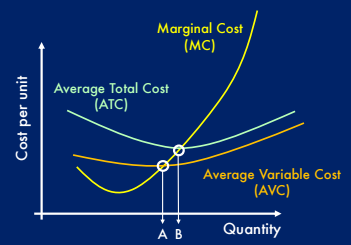
\includegraphics[width=.5\textwidth]{physicalCostCurve.PNG}
    \caption{Cost Curve for a Product of a Physcial Retailor}
  \end{figure}

  \begin{definition}{Business Supply Curve}
    A business's \textit{Supply Curve} is the minimum price-per-unit it is willing to sell each quantity of product at. It tends to be upwards sloping as marginal cost increases with quantity. The \textit{Supply Curve} will be truncated and not have a value for small quantities (in practice) as the business would fail if it sold too few products.
  \end{definition}

  \begin{definition}{Market Supply Curve}
    The \textit{Market Supply Curve} is the total number of units available, for a given price, across all producers in a market.

    \par The area above the \textit{Market Supply Curve} and below the \textit{Market Price} is the \textit{Producer Surplus}. This is the total additional income a producer receives after costs (i.e. total profit). Producers want to maximise \textit{Producer Surplus}
  \end{definition}

  \begin{definition}{Competitive Equilibrium}
    In a \textit{Competitive Market} the \textit{Market Equilibrium Price} will be that where the \textit{Consumer Demand Curve} and \textit{Market Supply Curve} intersect, as this is the price where quantity demanded and supplied are equal. The \textit{Market Equilibrium Price} maximises total surplus for both consumers and producers.
  \end{definition}

  \begin{definition}{Shifts}
    \textit{Shifts} can occur which move the whole of a supply or demand curve. These occur from non-price factors. e.g. a pandemic will cause a shift in the demand curve for face masks. These will cause a shift in  \textit{equilibrium price}.
  \end{definition}

  \begin{definition}{Monopoly Market}
    A market is considered a \textit{Monopoly} if its structure is characterised by a single seller (The \textit{Monopolist}). The \textit{Monopolist} faces no competition and thus can be a price \underline{setter}, rather than price taker. In the real world a firm with over 40\% market share is considered to have a monopoly. Monopoly markets are not competitive.
  \end{definition}

  \begin{definition}{Pareto Efficiency}
    An allocation is \textit{Pareto Efficient} if no-one can be made better-off without someone else being made worse-off. Pareto efficient allocations can arise from free markets, despite traders acting only to serve themselves (the \textit{invisible hand} guides them).
    \par Free markets are not \textit{guaranteed} to achieve optimal allocations. Some conditions under which this fails are well known (e.g. monopolies).
  \end{definition}

\subsection{Elasticity}

  \begin{definition}{Price Elasticity of Demand}
    \textit{Price Elasticity} is a measure of the how much the price of a product affects the quantity demanded. The more horizontal the demand curve, the greater the quantity demanded increases for a given decrease in price, (i.e. the more elastic the price is).
    \begin{itemize}
      \item A \textit{Horizontal} demand curve has \textit{Perfect Price Elasticity} as a change in quantity has no affect on price.
      \item A \textit{Vertical} demand curve has \textit{Perfect Price \underline{In}elasticity} as a fix quantity is demanded, at any price.
      \item A \textit{45 degree} demand curve has \textit{Unit Price Elasticity} as an $\Delta\%$ change in supply will produce an $\Delta\%$ change in demand.
    \end{itemize}
  \end{definition}

  \begin{definition}{Price Elasticity of Supply}
    \textit{Supply Elasticity} is a measure of how much a change in quantity supplied will affect the cost of production. The more horizontal the \textit{Supply Curve} is the less the price of production increases for a given quantity.
    \begin{itemize}
      \item A \textit{Horizontal} demand curve has \textit{Perfect Price Elasticity} as a change in quantity has no affect on price.
      \item A \textit{Vertical} demand curve has \textit{Perfect Price \underline{In}elasticity} as a fix quantity is demanded, at any price.
      \item A \textit{45 degree} demand curve has \textit{Unit Price Elasticity} as an $\Delta\%$ change in supply will produce an $\Delta\%$ change in demand.
    \end{itemize}
  \end{definition}

\subsection{Price Discrimination}

  \begin{definition}{Price Discrimination}
    \textit{Price Discrimination} is the practice of charging different prices to different customers for the same product. There are three levels of price discrimination
    \begin{itemize}
      \item[$1^\text{st}$ Degree]  \textit{Personalised} pricing. The business charges the maximum possible price for each unit sold (perfect price discrimination).
      \item[$2^\text{nd}$ Degree]  Product \textit{versioning} or \textit{menu pricing}. A company charges a different price for different quantities/qualities (ie bulk discount). Consumers have a choice over which version they buy, and thus the price. Here the discrimination depends on the product bought, rather than on characteristics of the customer, and encourages customers to self-select/
      \item[$3^\text{rd}$ Degree]  \textit{Group} pricing. The business charges a different price to different customer groups (e.g. age,location). The consumer does not get to choose their group. The groupings try to separate customers by their \textit{price elasticity} (The more price elastic charged less).
    \end{itemize}
    See \texttt{Figure 3}

    \begin{figure}[ht!]
      \centering
      \begin{subfigure}[b]{.3\textwidth}
           \centering
           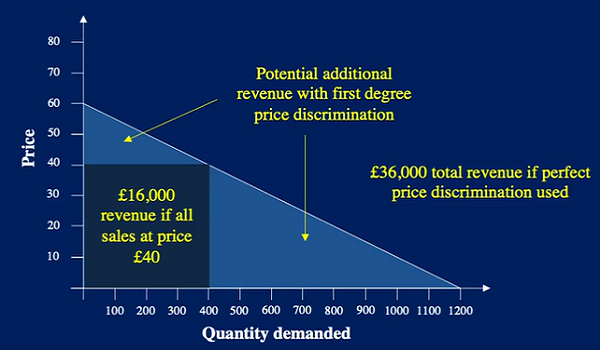
\includegraphics[width=\textwidth]{personalisedPricing.PNG}
           \caption{$1^\text{st}$ Degree}
      \end{subfigure}
      \begin{subfigure}[b]{.3\textwidth}
          \centering
          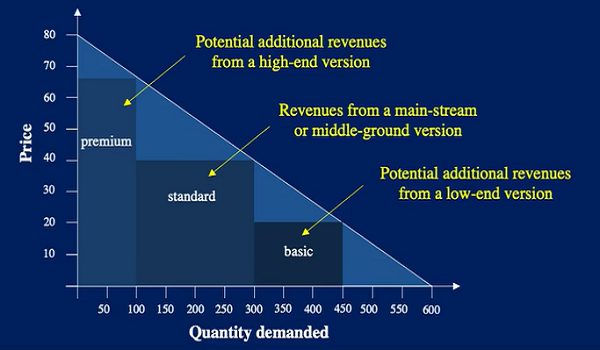
\includegraphics[width=\textwidth]{versioningPricing.PNG}
          \caption{$2^\text{nd}$ Degree}
      \end{subfigure}
      \begin{subfigure}[b]{.3\textwidth}
           \centering
           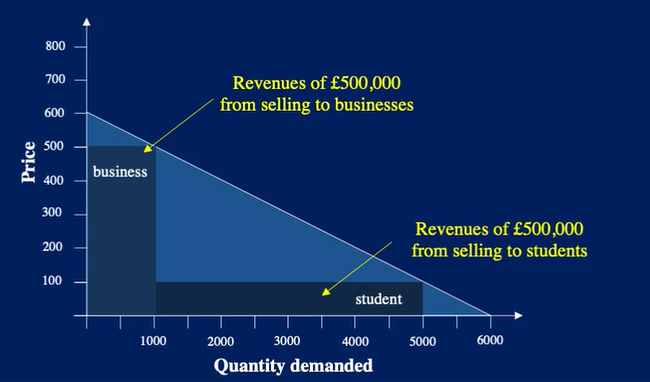
\includegraphics[width=\textwidth]{groupPricing.PNG}
           \caption{$3^\text{rd}$ Degree}
       \end{subfigure}
      \caption{Potential revenue increases for different pricing strategies}
    \end{figure}

  \end{definition}

  \begin{proposition}{Requirements for Price Discrimination}
    For a seller to be able to effectively price discriminate they must fulfil the following
    \begin{enumerate}
      \item Be able to \textit{distinguish between customers} so as to know what price to charge them.
      \item Have enough \textit{market power} to be able to set prices above marginal costs.
      \item \textit{Resale} must be impractical to prevent arbitrage.
    \end{enumerate}
    It is generally easier for online business to meet these criteria.
  \end{proposition}

  \begin{remark}{Loyalty Schemes}
    Loyalty schemes can be considered $2^\text{nd}$ degree price discrimination. Loyalty schemes can be a useful way of profiling customers and thus contributes to other forms of price discrimination.
  \end{remark}

  \begin{definition}{Price Steering}
    \textit{Price Steering} is when search results are personalised to place more/less expensive results at the top of the list. This encourages customers to spend at that price point due to placing an anchor, but the customer is still free to choose any product.
  \end{definition}

  \begin{definition}{Net Utility}
    The \textit{Net Utility} of a product to a consumer is the difference between the price of the product and the consumer's perceived value of the product. (e.g. If a product is sold at £5 but a consumer values it at £7, the net utility is £7-£5=£2). It is assumed a customer will never by a product that has a \textit{negative net utility} to them.
  \end{definition}

  \begin{example}{Economics of Versioning}
    Suppose we have a product priced at £10. Consider two customers: \textit{addict} who values it at £20; and \textit{casual} who values it at £8. The company will sell a single unit (to \textit{addict}) at £10.
    \par Now, suppose the company brought in a \textit{cut-down} version at £5 which \textit{addict} values at £8; and the casual user at £7. The company will now sell one full product (to \textit{addict}) and one \textit{cut-down} product (to \textit{casual}) for a total of £15.
    \par In fact, pricing the \textit{cut-down} version at £7 and the \textit{full} version at £19 would maximise profit (assuming customers go for the superior product when they have the same net utility for both) as this would be a perfect price for  \textit{casual} and the net utility is the same (£1) for \textit{addict} for both products.
  \end{example}

  \begin{proposition}{Competing against Yourself}
    A risk of versioning is that consumers who are willing to pay for the higher price, will choose to pay for the lower price one (due to greater net-utility). Thus choosing pricing points \& functionalities is therefore critical to business success.
  \end{proposition}

  \begin{proposition}{Bundling}
    \textit{Bundling} is a form of \textit{versioning} where several goods are sold together for a single price. (e.g. microsoft office). Bundling is used to sell customers products they would not otherwise buy. Bundling can create barries to entry for competitor producers as it requires competitors to produce a wider varity of product (e.g. a spreadsheet software \& word processor rather than just one).
  \end{proposition}

\section{Economic Agents}

  \begin{definition}{Bull \& Bear}
    An asset is described as \textit{Bullish} if its value is expected to \underline{increase}; Or, \textit{Bearish} if its value is expected to \underline{decrease}.
  \end{definition}

  \begin{remark}{CDA Curves in Practice}
    The supply and demand curves for continuous-action double auctions are, in reality, stepped. This is due to the relatively few units for sale in the market
  \end{remark}

  \begin{figure}[ht!]
    \centering
    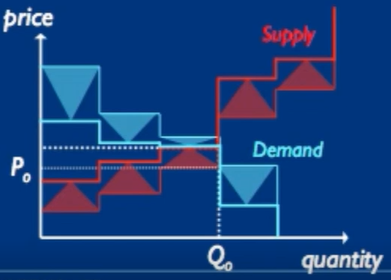
\includegraphics[width=.3\textwidth]{quotedPrices.PNG}
    \caption{The arrows show the displacement from an agents hidden price and their quoted price}
  \end{figure}

  \begin{proposition}{No-one Trades their Marginal Price}
    In practice sellers do not want to sell at their marginal price, nor do buyers want to buy at their maximum price. To avoid this both are advised to start a little away from these prices. These offered prices are known as \textit{Quote Prices}. Quoted prices have their own \textit{apparent} supply and demand curves which may be very different from the true curves. (See \texttt{Figure 4} ).
    \par The distance between the apparent and actual curves gives you the margin that agents are trying to achieve in the market. Agents should change their margin to reflect those of other people in the market. You would expect margins to decrease as the time since last transaction increases.
    \par Traders to the left of the equilibrium price can increase their margins to meet the equilibrium, while those on the right have to decrease.
  \end{proposition}

  \begin{proposition}{Dynamic Variation of Supply \& Demand Curves}
    In reality markets equilibriums are dynamic, as if the buyer and seller closest to the equilibrium perform a transaction they will drop out the market and a new equilibrium will need to be found. Also, new buyers and sellers may join the market. This is obvious in markets with very few units.
  \end{proposition}

  \begin{definition}{Experimental Economics}
    \textit{Experimental Economics} perform lab-style studies of human market-trading behaviours.
    \begin{itemize}
      \item A small number of human subjects are split into `buyers' and `sellers'.
      \item All traders are given a private-value/limit price which they cannot exceed.
      \item Traders interact within some market mechanism.
    \end{itemize}
    \textit{Experimental Economics} has demonstrated rapid equilibration in CDAs with very small number of traders.
  \end{definition}

\subsection{Metrics for Markets}

  \begin{definition}{Smith's $\alpha$}
    \textit{Smith's $\alpha$} is a measure of transaction price variation around the theoretical equilibrium price (as a percentage). Lower is better
    \[ \alpha:=\frac{100}{P_0}\sqrt{\sum_{t\in T}\frac{(P_t-P_0)^2}{|T|}} \]
    where $P_0$ is the equilibrium price and $\{P_t\}$ is the set of offered prices.
  \end{definition}

  \begin{definition}{Allocative Efficiency}
    \textit{Allocative Efficiency} is a measure of how effecitve the market is at extracting \textit{`gains through trade'}.
    \[ 100\times\frac{\text{Total utility earned by all traders}}{\text{Theoretical maximum possible total utility}} \]
  \end{definition}

  \begin{definition}{Single Agent Efficiency}
    \textit{Single Agent Efficiency} measures how well an individual agent performs.
    \[ 100\times\frac{\text{Profit Earned}}{\text{Expected profit all all trades done at }P_0} \]
  \end{definition}

  \begin{proposition}{Intelligence required for an allocative efficient CDA}
    How much of the allocative efficiency of a CDA is due to the intelligence of the traders> And how much is due to the organisation of the market?
    \par \textit{Experimental Economics} demonstrated (in 1993) than a zero-intelligence trading agent (ZIC) which quoted random prices (but constrained not to trade at a loss) is surprisingly human-like. Suggesting most of the intelligence is in the market, not in the traders.
  \end{proposition}

\subsection{Trading Algorithms}

  \begin{proposition}{How ZIC Traders achieve an equilibrium}
    \par ZI-C \textit{sellers} generate offer prices at random in a range from the lowest seller limit price $S_\text{min}$ and the maximum price allowed in the system $P_\text{max}$. This gives us a probability density function for offer prices which follows the supply curve.
    \par ZI-C \textit{buyers} generate offer prices at random in a range from the greatest buyer limit price $D_\text{max}$ and the minimum price allowed in the system $P_\text{min}$. This gives us a probability density function for bid prices which follows the demand curve.
    \par The intersection of these two distributions gives the distribution of prices at which transactions are done. See \texttt{Figure 5}. It is noteworthy that the expected values of these distributions are not equal as it means markets populated by ZIC traders achieve an equilibrium by chance (and will not reach an equilibrium in markets with assymetric supply and demand curves).
  \end{proposition}

  \begin{figure}[ht!]
    \centering
    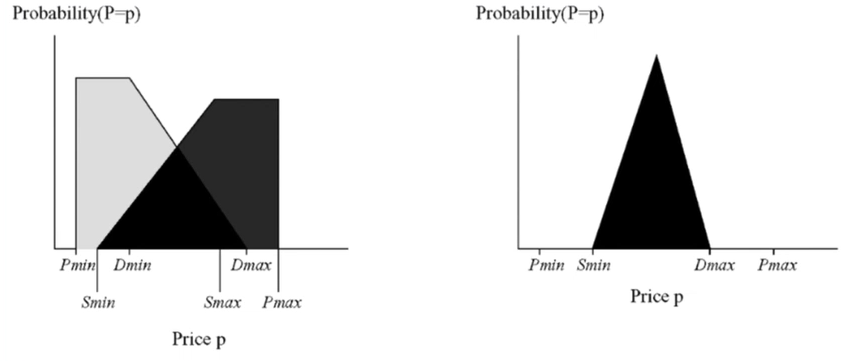
\includegraphics[width=.5\textwidth]{ZICTransactions.PNG}
    \caption{Distributions for offer, bid \& transaction prices for ZIC Traders}
  \end{figure}

  \begin{proposition}{ZIP Traders (1997)}
    \textit{ZI-Plus} (ZIP) Traders are a more advanced form of \textit{Zero-Intelligence Traders}. They still have a limit price which they cannot exceed, but also use machine learning in order to adapt. They have a \textit{profit margin} which is the distance between the price they quote and their limit price, this margin is adjusted by the machine learning over time.
    \par These have been shown to be much more human-like in CDA, than ZIC traders and achieves an equilibrium in cases where ZIC traders could not.
  \end{proposition}

  \begin{proposition}{ZIP Algorithm - Qualitative}
    The algorithm a ZIP trader uses is as follows.
    \par Consider a seller with limit price $L$. They will ask for a price $P:=L(1+M)$ where $M$ is some profit margin. If this price is \textit{accepted} then increase $M$; otherwise, decrease $M$.
    \par Buyers should do the inverse with their value of $M$.
    \par The amount to change $M$ by is determine by a \textit{learning rule} (e.g. Widrow-Hoff with Momentum).
  \end{proposition}

  \begin{proposition}{ZIP Algorithm - Quantitative}
    Let $\lambda_i$ denote the limit price of trader $i$; $p_i(t)$ denote the quote price of trader $i$ at time $t$; and $\mu_i(t)$ denote the profit margin of trader $i$ at time $t$. Then
    \[ p_i(t)=\lambda_i(1+\mu_i(t)) \]
    If $p_i(t)$ is accepted then $\mu_i(t+1)=\mu_i(t)+something$; otherwise; $\mu_i(t+1)=\mu_i(t)-something$ where the value of $something$ is determined by a stochastically determined \textit{Target price} and a learning rule aimed at achieving that price.
  \end{proposition}

  \begin{proposition}{ZIP Trader Target Price}
    The target price $\tau_i$ should be slightly beyond the last quoted price in the market $q(t)$.
    \[ \tau_i(t)=A_i(t)+q(t)R_i(t) \]
    where $R_i(\cdot)$ and $A_i(t)$ are stochastic functions for adjusting the last quoted price with $R_i(\cdot)$ being relative and $A_i(t)$ being absolute. These functions are defined by the learning rule.
  \end{proposition}

  \begin{definition}{Widrow-Hoff Learning Rule}
    The \textit{Widrow-Hoff} learning rule adjusts an observed value $A$ towards a desired value $D$, at rate $\beta$. The rule is defined as
    \[ A(t+1)=A(t)+\Delta(t)\quad\text{where}\quad\Delta_i=\beta\big(D(t)-A(t)\big) \]
    For ZIP a damping (momentum) factor $\gamma\in[0,1]$ is introduced
    \[ A(t+1)=\gamma A(t)+\Delta_i(t)(1-\gamma)\quad\text{where}\quad\Delta(t):=\beta\big(D(t)-A(t)\big) \]
    In the context of ZIP this is defined as
    \[ \mu_i(t+1)=\frac1{\lambda_i}(p_i(t)+\Delta_i(t))-1\quad\text{where}\quad\Delta_i(t):=\beta_i\big(\tau_i(t)-p_i(t)\big) \]
    Giving
    \[ \mu_i(t+1)=\frac1{\lambda_i}\big(p_i(t)+\Gamma_i(t)\big)-1\quad\text{where}\quad\Gamma_i(0):=0;\ \Gamma_i(t+1):=\gamma_i\Gamma_i(t)+\Delta_i(t)\big(1-\gamma_i\big) \]
  \end{definition}

  \begin{proposition}{Todd Kaplan's Sniper (1993)}
    Kaplan's \textit{Sniper Algorithm} is a robust and effective trading algorithm.
    \par The trader does nothing until the bid-offer spread drops to a sufficiently small value \underline{or} the offer is less than the smallest transaction price in the previous period \underline{or} there is only a short time until the market closes. When one of these conditions is fulfilled the trader jumps in, as long as the deal makes the sniper a profit greater than some threshold, and \textit{"snipes the deal"}.
    \par Note that this algorithm does adapt to the market, nor does it help prices converge to an equilibrium. Moreover, it relies on there being other ``more'' intelligent traders in the market for it to leech off.
  \end{proposition}

  \begin{proposition}{GD Traders (1998)}
    \textit{Gjerstad-Dickhaut} (GD) Traders using an algorithm which is based on producing a estimate of the probability of a certain price being accepted. This is defined by the trader's \textit{belief function} which uses data from the $n$ most recent market activity.
    \[ f(p)=\frac{able(p)+ole(p)}{able(p)+ole(p)+rgbe(p)} \]
    where $p$ is the price being queried, $able(p)$ is the number of accepted bids at prices less than $p$ in the last $n$; $ole(p)$ is the number of offers made below $p$ in the last $n$; and, $rgbe(p)$ is the number of rejected bids priced above $p$, in the last $n$.
  \end{proposition}

  \begin{proposition}{MGD Traders (2001)}
    MGD is a \textit{Modified} version of \textit{GD} with the follow considerations made:
    \begin{itemize}
      \item Use interpolation to smooth the function for prices which have not occurred in the market history.
      \item Choosing a quote-price which maximises the trader's expected gain (utility gain times probability of acceptance).
      \item Assign 0 probability for bids lower than previous lowest big, or offers above the previous greatest trade price.
    \end{itemize}
  \end{proposition}

  \begin{proposition}{GDX Traders (2002)}
    \textit{GDX} is another extension of \textit{GD} which uses real-time \textit{dynamic programming} to formulate agent bidding strategies in a broad class of auctions characterised by sequential bidding and continuous clearing.
  \end{proposition}

  \begin{proof}{Adaptive-Aggressive Algorithm (2006)}
    \textit{AA} Traders uses past history to adjust it's \textit{aggressiveness} (rather than profit margin) over time. \textit{Aggressiveness} quantifies how quickly it changes its pricing in response to market conditions.
    \par \textit{AA} Traders use an estimate of the current market equilibrium price $P_0$ (using past transactions) and \textit{Smith's $\alpha$} estimate of volatility to determine its level of aggression.
  \end{proof}

  \begin{proposition}{Deciding which algorithm to use}
    An analytical (game-theoretical) approach to choosing which trading algorithm is optimal is very hard and sometimes impossible. Some proofs require over simplifying assumptions which limit the end conclusion.
    \par Instead \textit{empirical studies} (simulation experiments) are used. This requires good \textit{"Design of Experiments"} and appropriate statistical analysis of results.
  \end{proposition}

  \begin{proposition}{Design of Experiments}
    \begin{itemize}
      \item \textit{Homogeneous Population Tests} assumes that all traders use the same algorithm. This is true in some cases (such as market-based resource allocation) but not many. This means only limited conclusions can be made.
      \item \textit{One-in-Many Test} have all but one member of a trading population using the same algorithm. This explores the vulnerability of the dominant algorithm, and the ability of the alternative algorithm to exploit the market. IRL, if the alternative algorithm was better you would expect some other traders to defect.
      \item \textit{Balanced-Group Test} have groups of equal size, each running a different algorithm but with matched limit prices. This is generally seen as the best test for comparing two different algorithms.
    \end{itemize}
    Simplex plots can be used to show the relationship between different ratio of traders.
  \end{proposition}

  \begin{remark}{The Best Algorithm}
    \begin{itemize}
      \item Balanced-Group Tests showed MGD to be superior to ZIC,ZIP \& GD in all cases.
      \item Balanced-Group Tests AA was shown to out perform GDX \& ZIP, in most cases. (Importantly AA is not dominant)
    \end{itemize}
    There are likely to be unpublished algorithms which out perform these.
  \end{remark}

\subsection{Empirical Methods}

  \begin{remark}{When to use a $t$-Test}
    A \textit{$t$-Test} can only be used when it is safe to assume that the underlying distribution is a normal distribution. There are tests of normality to check this.
  \end{remark}

  \begin{proposition}{$A-B$ Test}
    Here I describe a test to determine whether some method $A$ is better than some method $B$.
    \begin{itemize}
      \item Calculate the confidence interval on mean of samples from $A$.
      \item Calculate the confidence interval on mean of samples from $B$.
      \item If the intervals do not overlap then we can determine that one method is better than the other.
    \end{itemize}
  \end{proposition}

  \begin{definition}{Wilcoxon-Mann-Whitney U Test}
    The \textit{Wilcoxon-Mann-Whitney U Test} is a powerful test for two independent samples on a continuous dependent variable. It is a \textit{non-parameteric} version of the $t$-test. This test makes some assumptions, see \texttt{Proposition }
    \par Let $A$ be a sample of size $n_A$ and $B$ be a sample of $n_B$, with $n_A>n_B$.
    \begin{center}$H_0$: $A$ and $B$ come from the same population.\\$H_1$: $A$ and $B$ come from \textit{different} populations\end{center}
    \begin{enumerate}
      \item Combine $A$ and $B$ into one list and sort it (keeping track of which data point is from which sample).
      \item Rank the list from lowest to highest. Awarding average rank when ties occur.
      \item Sum the ranks for $A$ and $B$ to get $R_A,R_B$.
      \item Compute $U_B:=n_An_B+\frac12n_A(n_A+1)-R_A$ and $U_B:=n_An_B+\frac12n_B(n_B+1)-R_B$.
      \item Define $U:=\min\{U_A,U_B\}$.
      \item Compare $U$ to the critical value from $U_{n_A,n_B,\alpha}$ from a lookup table.
      \item If $U<U_{n_A,n_B,\alpha}$ then reject $H_0$.
    \end{enumerate}
    The \textit{U-Test} is a pairwise test, but it is bad to performance a series of these tests as the error grows quickly. (ie If you are testing at a siginifance level of $95\%$, the probability of being correct after four tests is $.95^4=.814...$)
  \end{definition}

  \begin{proposition}{Assumptions of U Test}
    \begin{itemize}
      \item The Independent variable data is in two groups (Control and Treatment).
      \item The dependent variable is at least in an ordinal scale.
      \item Data is randomly selected samples from the two groups
      \item The population distributions of the dependent variable for the two groups have a similar shape, but have differences in measures of central tendency.
    \end{itemize}
  \end{proposition}

  \begin{definition}{Kruskal-Wallis Test}
    The \textit{Kruskal-Wallis Test} is a generalisation of the \textit{U Test}, extending it to allow multiple group comparisions.
    \par Consider samples $A,B,C,D$
    \begin{enumerate}
      \item Calculate the mean ranking for each group's entries in the sorted union list. (As in U Test)
      \itme Compute a statistic H form the mean rank and the sample size $n$.
      \item Use a $\chi^2$-test to determine whether $H$ is significant.
    \end{enumerate}
  \end{definition}

\subsection{Options Markets}

  \begin{definition}{Short Selling}
    To \textit{Short} a stock, is when you borrow a stock from someone else and sell the borrowed stock immediately. You will then need to buy a stock at some point in the future to return to the original lender, ideally for less than you sold the borrow stock for.
    \par \textit{Shorting} can be used as insurance against other market events.
  \end{definition}

  \begin{definition}{Derivative}
    A \textit{Derivative} contract is based on the \textit{marginal change} in value of an asset. They do not require you to buy/own an actual stock, rather you work on the \textit{margin} of the stock. There are different types of \textit{Derivative}
    \begin{itemize}
      \item A \textit{Futures} contract is one which \underline{must} be executed by/on a set \textit{delivery} date. A \textit{Forward price} is defined when the contract is issued, and this is the price the final transaction will occur at. Common for selling crop yields.
      \par Buyers of a forward have the \textit{long position} and sellers have the \textit{short position}.
      \item An \textit{Options} contract is one which \underline{may} be executed by/on a set \textit{delivery} date. There is no obligation. \textit{Options} have a \textit{Strike price} which is the price which the transaction will be done at, if a transaction is done at all.
      \par Options to sell are called \textit{puts} and options to buy are \textit{calls}.
    \end{itemize}
    The option is said to be \textit{written} by the seller and \textit{held} by the buyer.
  \end{definition}

  \begin{remark}{Futures and Options}
    Both futures and options are
    \begin{itemize}
      \item \textit{Standardised}. The size of the contract and the delivery/expiry date are prespecified.
      \item \textit{Exchange Traded}. The contracts can be bought and sold on a secondary market. This is required so that those who do not have enough money to actually exercise the full value of their option can still realise the option's value, by selling to someone who can afford to exercise the option.
    \end{itemize}
  \end{remark}

  \begin{remark}{Price of an Option}
    The price of an option depends on the
    \begin{itemize}
      \item \textit{Intrinsic Value}. The money received if the option is exercised now.
      \item \textit{Volatility Premium}. The volatility in price of the underlying asset.
      \item \textit{Time Value}. The potential risk-free return on money saved wrt buying the underlying asset. (ie what you could received if the money was placed in a safe investment, rather than the option)
    \end{itemize}
  \end{remark}

  \begin{definition}{American-Style \& European-Style}
    An \textit{American-Style} option can be exercised on any date up to the expiry date.
    \par A \textit{European-Style} option can \underline{only} be exercised on its expiry date.
  \end{definition}

  \begin{definition}{Call Option}
    A \textit{Call option} gives the holder the right to buy $N$ units of the underlying asset, at some point in the future, at a specified \textit{Strike Price}. If exercised the option-write (Seller) must sell the $N$ shares at the strike price.
    \par The \textit{Call Option} is \textit{In The Money} (ITM) if the underlying asset price is greater than the strike price; \textit{Out The Money} (OTM) if the underlying price is less than the strike price; Or, \textit{At The Money} if the underlying price equals the strike price.
  \end{definition}

  \begin{definition}{Put Option}
    A \textit{Put Option} gives the hold the right to sell $N$ units of the underlying asset, at some point in the future, at a specified \textit{Strike Price}. If exercised the option-writer (Seller) must buy the $N$ shares at the strike price.
    \par The \textit{Call Option} is \textit{In The Money} (ITM) if the underlying asset price is less than the strike price; \textit{Out The Money} (OTM) if the underlying price is greater than the strike price; Or, \textit{At The Money} if the underlying price equals the strike price.
  \end{definition}

  \begin{remark}{Commissions are paid on setting up option contracts.}

  \end{remark}

\subsubsection{Option Strategies}

  \begin{proposition}{Option Strategies}
    \textit{Option Strategies} are linear combinations of options:
    \begin{itemize}
      \item Long call
      \item Short call
      \item Long put
      \item Short put
    \end{itemize}
  \end{proposition}

  \begin{figure}[ht!]
    \centering
    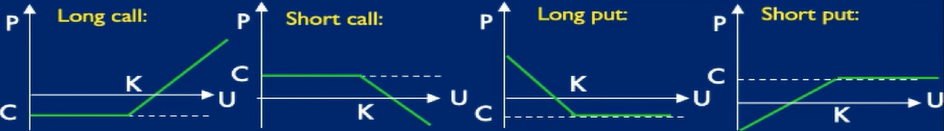
\includegraphics[width=.5\textwidth]{options.PNG}
    \caption{Different Basic Option Pay Off Diagrams}
  \end{figure}

  \begin{definition}{Bull Spread}
    A \textit{Bull Spread} is an option strategy which bounds the pay off to a constant, this limits the risk by placing a cap on potential losses. A \textit{Bull Spred} is made up of a \textit{Long call at $K_1$} and a \textit{Short Call at $K_2$} (Bullish Call Spread); or the same but with \textit{put} options (Bullish Put Spread). In practice the losses are limited to the $K_2$ price as if the underlying price was to exceed $K_2$ then you would exercise the short option.
  \end{definition}

  \begin{figure}[ht!]
    \centering
    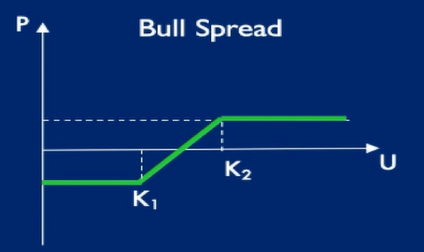
\includegraphics[width=.5\textwidth]{bullSpread.PNG}
    \caption{Bull Spread Pay off Diagram}
  \end{figure}

  \begin{definition}{Bear Spread}
    A \textit{Bear Spread} is an option strategy which bounds the pay off to a constant, this limits the risk by placing a cap on potential losses. A \textit{Bear Spred} is made up of a \textit{short put at $K_1$} and a \textit{long put at $K_2$} (Bearish Put Spread); or the same but with \textit{call} options (Bearish Call Spread). In practice the losses are limited to the $K_2$ price as if the underlying price was to fall below $K_2$ then you would exercise the long put option.
  \end{definition}

  \begin{figure}[ht!]
    \centering
    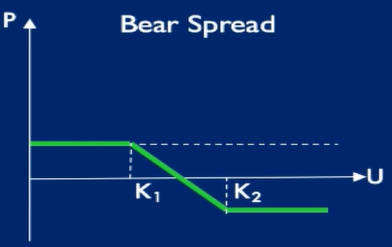
\includegraphics[width=.5\textwidth]{bearSpread.PNG}
    \caption{Bear Spread Pay Off Diagram}
  \end{figure}

  \begin{definition}{Long Butterfly}
    A \textit{Long Butterfly} strategy is used when you expect the price not to change much. A \textit{Long Butteryfly} is made up of a \textit{Long Call at $K_1$}, two \textit{Short calls} each at $K_2$, and another \textit{Long Call at $K_3$}
  \end{definition}

  \begin{figure}[ht!]
    \centering
    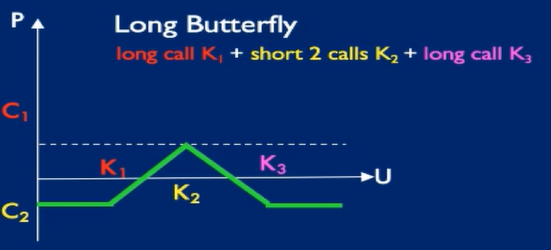
\includegraphics[width=.5\textwidth]{longButterfly.PNG}
    \caption{Long Butterfly Pay Off Diagram}
  \end{figure}

  \begin{definition}{Short Butterfly}
    A \textit{Short Buterfly} strategy is used when you expect the price of an asset to change (in either direction) from its current value. A \textit{Short Butterfly} is made up of: a \textit{Short Call at $K_1$}, two \textit{Long Calls} each at $K_2$ and another \textit{Short Call} at $K_3$.
  \end{definition}

  \begin{figure}[ht!]
    \centering
    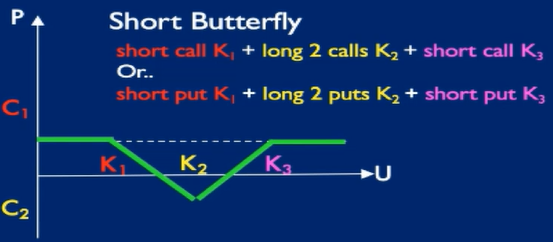
\includegraphics[width=.5\textwidth]{shortButterfly.PNG}
    \caption{Short Butterfly Pay Off Diagram}
  \end{figure}

  \begin{definition}{Long Straddle}
    A \textit{Long Straddle} strategy has an unbounded payoff, provided the value of the asset moves from its original value (Essentially an unbounded Long Butterfly). A \textit{Long Straddle} is comprised of a \textit{Long Call at $K_1$} and a \textit{Long Put at $K_1$}.
  \end{definition}

  \begin{figure}[ht!]
    \centering
    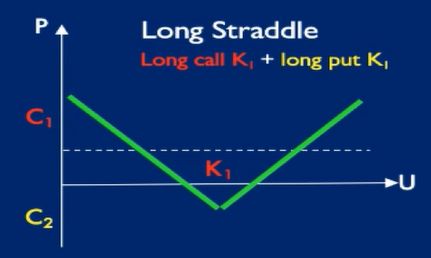
\includegraphics[width=.5\textwidth]{longStraddle.PNG}
    \caption{Long Straddle   Pay Off Diagram}
  \end{figure}

  \begin{definition}{Short Straddle}
    A \textit{Short Straddle} strategy has an unbounded payoff, provided the value of the asset does not move from its original value (Essentially an unbounded Short Butterfly). A \textit{Short Straddle} is comprised of a \textit{Short Call at $K_1$} and a \textit{Short Put at $K_1$}.
  \end{definition}

  \begin{figure}[ht!]
    \centering
    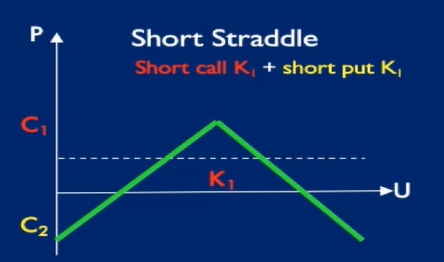
\includegraphics[width=.5\textwidth]{shortStraddle.PNG}
    \caption{Short  Straddle Pay Off Diagram}
  \end{figure}

  \begin{definition}{Long Strangle}
    A \textit{Long Strangle} strategy pays out provided the underlying asset values moves at least some specified amount from its original value (Essentially a long straddle which doesn't just meet at a point). A \textit{Long Strangle} is made up of a \textit{Long Put at $K_1$} and a \textit{Long Call at $K_2$}.
  \end{definition}

  \begin{figure}[ht!]
    \centering
    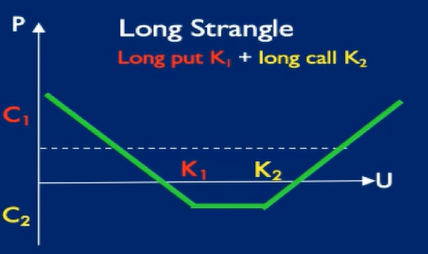
\includegraphics[width=.5\textwidth]{longStrangle.PNG}
    \caption{Long Strangle  Pay Off Diagram}
  \end{figure}

  \begin{definition}{Ratio Call Spread}
    A \textit{Ratio Call Spread} is similar to a long butterfly, but is unbounded in terms of losses should the underlying value keep increasing. A \textit{Ratio Call Spread} requires three options (One less than a \textit{Long Butterfly} so is cheaper): A \textit{Long Call at $K_1$} and two short calls, both at $K_2$.
    \par A \textit{Ratio Call Spread} is used when you are confident $U$ will rise to $K_2$, but no go beyond that.
  \end{definition}

  \begin{figure}[ht!]
    \centering
    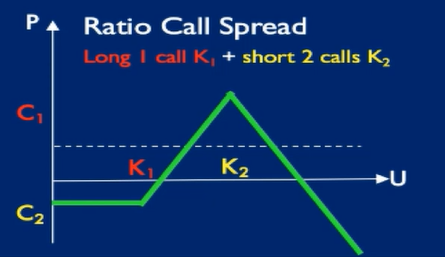
\includegraphics[width=.5\textwidth]{ratioCallSpread.PNG}
    \caption{Ratio Call Spread Pay Off Diagram}
  \end{figure}

  \begin{definition}{Ratio Put Spread}
    A \textit{Ratio Put Spread} is similar to a long butterfly, but is unbounded in terms of losses should the underlying value keep decreasing. A \textit{Ratio Put Spread} requires three options (One less than a \textit{Long Butterfly} so is cheaper):  Two \textit{Short Puts at $K_1$} and a long put at $K_2$.
    \par A \textit{Ratio Put Spread} is used when you are confident $U$ will fall to $K_1$, but no go beyond that.
  \end{definition}

  \begin{figure}[ht!]
    \centering
    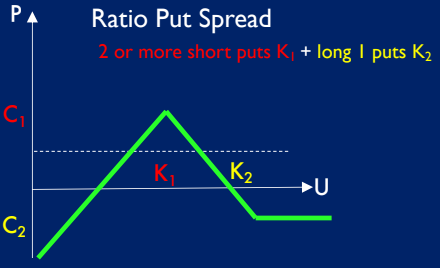
\includegraphics[width=.5\textwidth]{ratioPutSpread.PNG}
    \caption{Ratio Put Spread Pay Off Diagram}
  \end{figure}

  \begin{definition}{Ratio Call Backspread}
    A \textit{Ratio Call Backspread} is similar to a short butterfly, but is unbounded in terms of gains should the underlying value keep increasing. A \textit{Ratio Call Backspread} requires three options (One less than a \textit{Long Butterfly} so is cheaper):  A \textit{Short Call at $K_1$} and two \textit{Long Calls at $K_2$}.
    \par A \textit{Ratio Put Backspread} is used when you are confident $U$ will shift significantly, with an increase more likely.
  \end{definition}

  \begin{figure}[ht!]
    \centering
    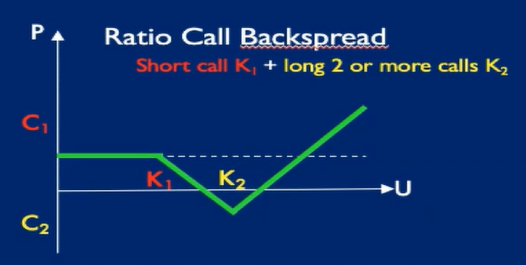
\includegraphics[width=.5\textwidth]{ratioCallBackspread.PNG}
    \caption{Ratio Call Backspread Pay Off Diagram}
  \end{figure}

  \begin{definition}{Ratio Put Backspread}
    A \textit{Ratio Put Backspread} is similar to a short butterfly, but is unbounded in terms of gains should the underlying value keep decreasing. A \textit{Ratio Put Backspread} requires three options (One less than a \textit{Long Butterfly} so is cheaper):  A \textit{Short Put at $K_1$} and two \textit{Long Put at $K_2$}.
    \par A \textit{Ratio Call Backspread} is used when you are confident $U$ will shift significantly, with an decrease more likely.
  \end{definition}

  \begin{figure}[ht!]
    \centering
    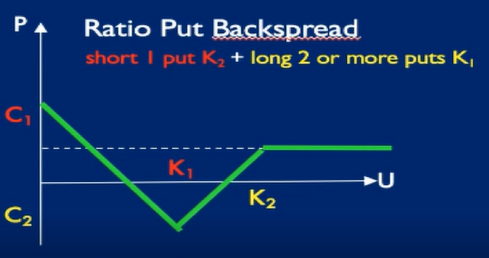
\includegraphics[width=.5\textwidth]{ratioPutBackspread.PNG}
    \caption{Ratio Put Backspread Pay Off Diagram}
  \end{figure}

  % \subsection{Betting Exchanges}

  \begin{proposition}{Betting Exchanges}
    \textit{Betting Exchanges} are similar to \textit{Options Markets} as they allow people who have differing views over some future outcome to wager on it. \textit{Betfair} offer a LOB style way to place bets by allowing users to \textit{"back"} (will happen) an event or \textit{"lay"} (will not happen) an event.
  \end{proposition}

\section{The Economics of The Internet}

  \begin{definition}{Network Externalities}
    A \textit{Network Externality} is an \textit{Externality} that occurs when the act of buying a product/serivce has an indirect cost or benefit to those who already own the same product/service. Products with \underline{positive} network externalities are often known as \textit{Network Goods}.

    \par Owning a mobile phone has a positive network externality as you are increasing the number of contactable people. Owning a car has a negative network externality as you increase road traffic.

    \par Positive network externalities can produce a \textit{Positive Feedback Loop} where people by products which are compatible with their friends, rather than necessarily the best product. This is part of \textit{Brand Value}.
  \end{definition}

  \begin{definition}{Network Effect Demand Curve}
    We can plot a \textit{Network Effect Demand Curve} (\texttt{Figure 3}) of the price customers are willing to pay against network size. This is slope upwards initially as the marginal value of each extra user is higher; eventually it will slope downwards as these marginal gains diminish.

    \par For any given price there are three equilibrium points $q_0,q_1,q_2$ for network size. $q_1$ is deemed unstable, the \textit{`tipping point'}, as once the network is larger than $q_1$ it will naturally grow to $q_2$ (as there is a consumer excess) but whilst it is smaller it will shrink to $q_0$ (as there is a consumer deficit). This means $q_1$ is the \textit{Critical Mass} for the network to be sustainable.
  \end{definition}

  \begin{figure}[ht!]
    \centering
    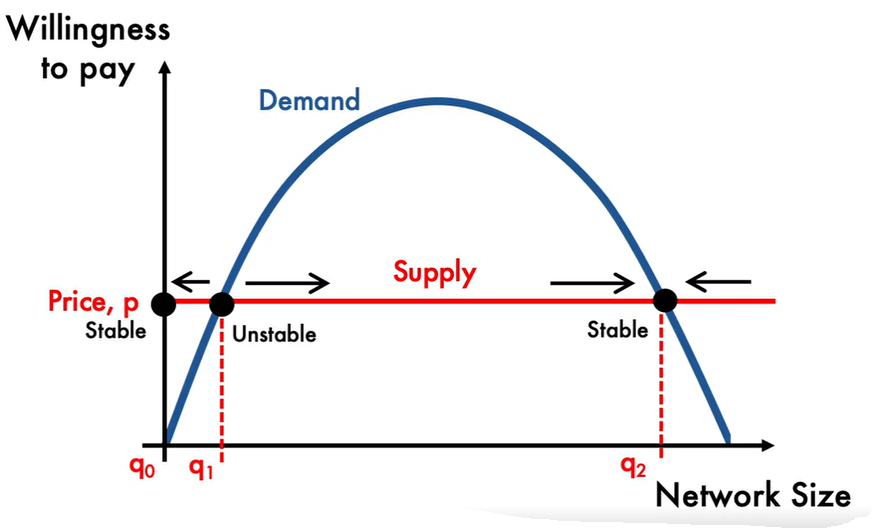
\includegraphics[width=.5\textwidth]{networkDemandCurve.PNG}
    \caption{Network Effect Demand Curve}
  \end{figure}

  \begin{proposition}{The Long Tail}
    Sales business typically sell either: high volume, low margin goods (e.g. burgers); Or, low volume, high margin goods (e.g. cars). Physcial sales businesses are constrained by the physical shelf space they have and thus avoid low volume, low margin goods. This means that the sales distribution for products in a physical store will be a truncated \textit{Pareto Distribution}.\\
    \par Internet businesses have unlimited shelf space to advertise products, and since warehouse space is much cheaper (per sq ft) they can store a lot more products for the same cost, effectively increasing the margin of each product. Meaning their are more products which are profitable to stock and the sales distribution for products of an internet business will have a much longer tail. (See \texttt{Figure 1}).
  \end{proposition}

  \begin{figure}[ht!]
    \centering
    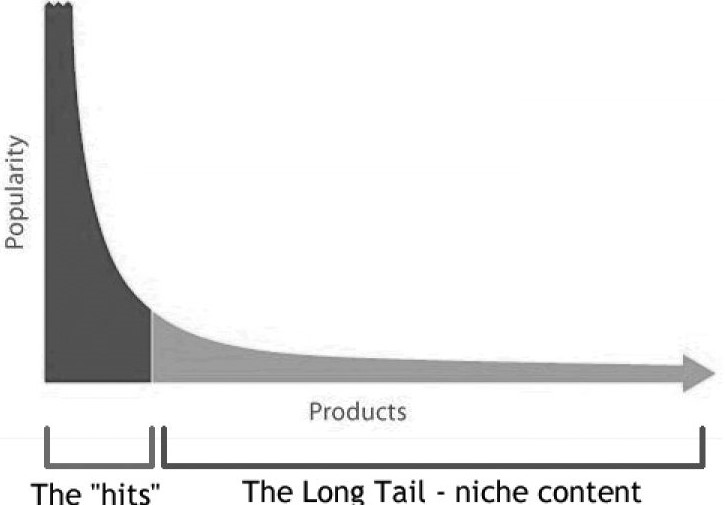
\includegraphics[width=.5\textwidth]{LongTail.jpg}
    \caption{The Long Tail}
  \end{figure}

  \begin{remark}{How to take advantage of `The Long Tail'}
    \begin{enumerate}
      \item Make everything available.
      \item Reduce prices (due to economies of scale \& reduced costs).
      \item Help customers find new products.
    \end{enumerate}
  \end{remark}

  \begin{remark}{Sustaining v. Disruptive Innovations}
    \textit{Sustaining Innovations} are those that incrementally improve existing products on traditional performance metrics. Eventually these will superceed customer requirements.
    \par \textit{Disruptive Innovations} perform less well on traditional performance metrics but sufficiently better along other metrics in order to generate new markets.
  \end{remark}

  \begin{proposition}{Disruptive Technology}
    Established companies are often late to invest in new \textit{disruptive} technologies. Typically this is due to the \textit{disruptive} tech not reaching the requirements of their customers. However, the \textit{disruptive} tech maybe better in other ways (lighter, more durable etc.) and so can establish a sufficient market for startups to invest in it. Once the \textit{disruptive} tech does reach the requirements of mainstream customers, they are likely to jump to the new tech for these bonus features (lighter, more durable etc.) and the established company may fail.
    \par The new tech may still be less powerful than the established tech, but it is sufficient for customers so it doesn't matter. The traditional performance metric for performance will vary by industry (e.g. mb/£ for hard drives).
  \end{proposition}

  \begin{proposition}{Timeline of Disruptive Technology}
    \begin{enumerate}
      \item \textit{Disruptive Technology} is invent. Often by an established company.
      \item The \textit{disruptive technology} does not meet established the established company's requirements and so not focused on.
      \item New companies form to pursue the \textit{disruptive technology}. Often by ex employees of the established company.
      \item \textit{Disruptive Technology} improves \& meets traditional performance metric requirements. The established company will likely try to enter the new market at this point but will be too late.
      \item \textit{Disruptive Technology} becomes the main stream.
    \end{enumerate}
  \end{proposition}

  \begin{proposition}{How to spot Disruptive Technology}
    \begin{enumerate}
      \item \textit{Determine whether the technology is disruptive or sustaining}
    \end{enumerate}
  \end{proposition}

\subsection{Properties of Online Businesses}

  \begin{remark}{Economic Laws}
    The \textit{Economic Laws} are not fundamentally different between online \& irl businesses, but the characteristics of online business activities can result in different markets.
  \end{remark}

  \begin{definition}{Combinatorial Innovation}
    \textit{Combinatorial Innovation} describes a technology who's components can be combined \& recombined to create new products and services. The Internet is a \textit{Combinatorial Innovation} due to its standardised and open-source nature.
  \end{definition}

  \begin{proposition}{Economic Differences between Digital \& Physical Goods}
    \begin{itemize}
      \item Digital goods tend to be costly to produce; but \textit{cheap to reproduce}. (i.e. Fixed costs are high but variable costs are low).
      \item Production costs for digital goods are \underline{sunk} costs. (e.g. You can sell a building you don't need, but cannot get money back from a software developer).
      \item There are \textit{no capacity constraints} limiting the number of times something can be reproduced.
      \item Digital goods are often \textit{Experience Goods}. (i.e. a customer will no know whether they will like it before they try it, and thus cannot assign a value to it).
      \item \textit{Serach Costs} for a consumer are very low. It is easy for consumer to compare products are go with the best. IRL this is harder as it requires going to different stores.
      \item Digital goods have \textit{strong positive network externalities}
    \end{itemize}
  \end{proposition}

  \begin{remark}{Switching Costs}
    A customer may incur a cost (inc. non-monetary) to switch services. This is more common (and costly) in the digital space than the physical. When switching costs are too high, consumers are \textit{locked in}. Possible switching costs include:
    \begin{itemize}
      \item Training cost.
      \item Network effects.
      \item Setup costs.
      \item Reduced service quality due to new provider not having all your information (consider switching from Netflix).
    \end{itemize}
  \end{remark}

  \begin{proposition}{Cost Curve for Digital Goods}
    Since digital goods have high fixed cost but low variable costs their \textit{cost curves} are very different. The \textit{Marginal Cost Curve} is effectively zero for all quantities; Average Variable Costs are effectively zero for all quantities; and, average total costs tend asymptotically towards zero.
    \par This means it is easy for an online business to survive in the short term and the minimum price they are willing to sell a product at is zero (due to v. low variable costs). Eventually the company will need to pay off its fixed costs.
  \end{proposition}

  \begin{figure}[ht!]
    \centering
    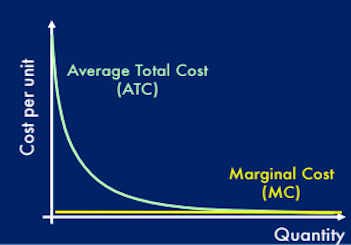
\includegraphics[width=.5\textwidth]{digitalCostCurve.PNG}
    \caption{Consumer Surplus \& Expenditure}
  \end{figure}

  \begin{remark}{Competition between Digital Companies}
    \begin{itemize}
      \item Due to low variable costs, companies with identical digital products will very quickly move prices to near-zero.
      \item New companies will struggle as fixed costs are high.
      \item Network effects \& switching costs make it hard for new companies.
    \end{itemize}
    Due to these \textit{barriers to entry} monopolies are common among digital companies. To succeed, a company needs to focus on product differentiation (i.e. innovation).
  \end{remark}

  \begin{remark}{Formats}
    Companies can make their software use \textit{Proprietary Formats}, meaning the files cannot be used by other software. This increases switching costs for customers.
    \par Using \textit{Industry-Wide Standards} allow a user's files to be shared between providers. This can increase the network effect, potentially attracting new customers. Here companies have a trade-off between having a large part of a small pie, or a small part of a large pie.
  \end{remark}

  \begin{remark}{How Standards Develop}
    \textit{Industry-Wide Standards} general develop in one of two ways
    \begin{enumerate}
      \item A \textit{single (major) player} sets a standard by opening up their proprietary format (e.g. PDF).
      \item A \textit{war} occurs between multiple standard setters. Generally detrimental to everyone involved.
      \item A \textit{negotiation} occurs between multiple standard setters. There is a risk that one party may pull out of the deal and use their own proprietary format.
    \end{enumerate}
  \end{remark}

\subsection{Price Discrimination Online}

  \begin{remark}{Personalised Pricing Online}
    \begin{itemize}
      \item Consumers tend perceive personalised pricing as \textit{unfair}.
      \item Consumers like \textit{transparency} (i.e. how a price is decided).
      \item European data protection laws \textit{require} companies inform people about the specific purpose of processing their personal data.
    \end{itemize}
  \end{remark}

  \begin{proposition}{Digital Product Versioning}
    \begin{itemize}
      \item Digital versions are used extensively and creatively as they are easy to prepare and near-zero cost to duplicate.
      \item Buyers have a choice over which version to buy, so do not find the practice controversial.
      \item \textit{Personalisation of Product} is an extreme typr of product versioning (becoming closer to $1^\text{st}$ degree price discrimination) as it allows user to specify many properties (e.g. screen quality, amount of ram \& storage for a pc).
      \item People tend to \textit{upsell} towards an ``almost top option'' when given a choice (the 2nd most expensive bottle of wine is often the most popular).
      \item Product versioning can cause you to \textit{compete with yourself} as some people who would have payed the higher price, will go for the lower price.
    \end{itemize}
  \end{proposition}

  \begin{remark}{Unbundling}
    \textit{Bundling} is common with physical software but there is also a practice of \textit{unbundling}. Since there is no physical substrate online there is less commercial pressure to bundle. (e.g. publishers can sell individual articles rather than a full magazine).
  \end{remark}

  \begin{remark}{'Free' Digital Versions}
    As the duplication cost of digital goods is almost zero, many are given away for free. In these cases there are still several ways for producers to make money: cut-down versions encourage you to buy a full version; Artificial delay (e.g. stock feeds); Ads (or pay for no adds).
    \par \textit{'Free'} versions allow a customer to build a truer valuation of a product, particularly useful for \textit{experience goods}.
    \par Even if a user is on the free model they are building the \textit{network effect} of the product and likely increasing the \textit{swapping costs} they will experience if they want to change product.
  \end{remark}

  \begin{proposition}{Freemium Model}
    The \textit{'Freemium'} business model is to offer different versions at different prices, \textit{including a free one}. The hope is a consumer will \textit{upgrade} to a paid version because they like the service.
  \end{proposition}

\subsection{Economics of Computer Games}

  \begin{proposition}{Virtual Game Economies}
    Virtual game economies are generally stimulated by players collecting raw materials and then producing goods which they sell between themselves, very much like an IRL economy.
    \par Virtual economies have many of the same issues as real economies. For a stable economy, a balance must be struck between currency sources (money entering) and skins (money leaving). If there is an imbalance then \textit{MUDflation} can occur (Multi-User-Dungeon inflation?). Designing these stable economies (for MMORPGs) is hard.
    \par Economic stability is important otherwise games can lose credibility. There are examples where players have developed \textit{meta currencies} which are more stable to improve a games longevity.
  \end{proposition}

  \begin{remark}{IRL Game Economies}
    There are real-world markets when players sell their in game items for IRL money. Essentially this a ForEX market.
  \end{remark}

  \begin{remark}{Gold Farming}
    As the value IRL market for a game's assets reaches it has been observed that people in developing nations will choose to grid the game (gold farm) in order to obtain items to then sell in an IRL market, rather than work a traditional job. This market is between the cash rich-time poor (americans) and cash poor-time rich (mexicans? sorry).
    \par This typically against a games EULA, but it is hard to game makers to counter.
  \end{remark}

  \begin{remark}{Game Development Budgets}
    The number of people involved in making a game and the number of lines in a typical AAA game has grown exponentially, tracking the powerfulness of computers.
    \par However, the \textit{average} game budge has decreased as many games as small titles made on tight budgets or as passion projects.
    \par Mid-size studios with projects budgets in the low millions are rare. This is typically due to either them being absorbed by bigger studios; or the mid-size studio breaks up into smaller teams.
    \par The rise in \textit{Content Costs} has increased due the number of many hours required to complete tasks and jobs have become much more specialised. Additional, game-developers now demand higher wages. Note that this is useful for big studios as they act as a barrier to entry.
  \end{remark}

\section{Auction Theory}

  \begin{remark}{Why Use Auctions?}
    \textit{Auctions} allow an item to be sold for a price which is wholely decided by a consumer's willingness to spend. \textit{Auctions} are a mechanism for first-degree \textit{price discrimination}, this makes them particulary popular online.
    \par Auctions are used when sellers are \textit{uncertain} about the value consumers place on an object (common with one off items). In this case auctions are good as they allow for \textit{price discovery}.
    \par Auctions are easy to automate and a form of differential pricing.
  \end{remark}

  \begin{proposition}{Auctions vs Posted Prices}
    When a seller chooses to run either an auction or use posted prices, they are choosing whether between \textit{price discovery} and \textit{convenience}. Auctions are often favoured by unexperienced sellers and unique items. Auctions sell for less than a posted price listing (otherwise consumers would pay the posted price listing).
  \end{proposition}

  \begin{definition}{Private Value}
    An object's \textit{Private Value} is the value each consumer places on the object. Each bidder knows their private value for an object, but do not know the private value of others nor does knowledge of other bidders' private values affect your private value. This situation is common for consumable goods, less so with investments.
  \end{definition}

  \begin{definition}{Interdependence}
    \textit{Interdependence} occurs when a bidder does know have a fixed value for an object and use other bids to improve their estimate of an objects value. This is common when other bidders may have more information.
  \end{definition}

  \begin{definition}{Open Auction}
    In an \textit{Open Auction} all bids are known to all particpants.
  \end{definition}

  \begin{remark}{Assumptions in Auction Theory}
    In Auction theory several assumptions are made:
    \begin{itemize}
      \item All auctions are equally attractive (ie there are no auctions where no one turns up);
      \item There is no collusion between bidders;
    \end{itemize}
    These assumptions means auction theory often does not work well in practice.
  \end{remark}

  \begin{remark}{Attendance at Auctions}
    Entering an auction can be quite involved, so often bidders will skip auctions they don't think they can win.
  \end{remark}

  \begin{definition}{Signalling}
    During an auction a bidder may place a \textit{`weird`} bid which signals their intent for the rest of the auction to other bidders. This is a form of collusion without any prior agreement necessary. (Consider the T-Mobile - Mannesbane auction for parts of the german telephone network).
  \end{definition}

  \begin{definition}{Reverse Auction}
    \textit{Reverse Auctions} are when multiple suppliers bid for a contract with a single consumer. This is commonly used for construction \& suppliment contracts, (inc. by governments).
    \par Often suppliers must be \textit{qualified} in order to \textit{offer} a price.
  \end{definition}

  \begin{definition}{Double Auction}
    In a \textit{Double Auction} multiple buyers and multiple sellers take part. The sellers offer descending prices, and buyers bid ascending prices. When two prices meet a sale is made between those two parties.
    \par \textit{Continuous Double Auctions} all buyers and sellers to place bids at any time, and not necessarily in order. This is used in stock exchanges.
    \par \textit{Double Auctions} are very efficient for price discovery.
  \end{definition}

  \begin{proposition}{Trading in the Dark}
    Sometimes you do not want to give away your private information (e.g. You dont want to list a large stock sale on a public order book as this would affect the stock price).
    \par \textit{Dark Pools} are designed to keep your trading intensions secret so that it does not impact price. WARNING it is common for dark pool owners to use this information against their users.
  \end{proposition}

  \begin{definition}{Posted Auction}
    A \textit{Posted Auction} is one where the seller posts a price and then buyers have an option to buy at that price (and that price alone). This is how most shops work.
  \end{definition}

\subsection{Open Auctions}

  \begin{definition}{English Auction}
    AKA \textit{Open Ascending-Price Auction}. Used in \textit{Homes under the Hammer}.
    \begin{enumerate}
      \item The auctioneer announces a (low) price to everyone.
      \item If a bidder is happy to pay that price they raise their hand. (Price is reduced if no one bids).
      \item Auctioneer will announce that that bidder is currently winning and will announce a new, higher price.
      \item ii)-iii) repeat until no-one accepts the new higher price (ie no hands are raised)
      \item The item is sold to the person who bid last, at the price of that last bid.
    \end{enumerate}
    Bidders can infer information from when others drop out of an auction. However, with \textit{Private Values} this will not change their strategy (it would for \textit{Interdependence}).
  \end{definition}

  \begin{proposition}{English Auction - Optimal Strategy}
    Let $v$ be the private value a bidder assigns to an object
    \begin{itemize}
      \item It is not optimal for a bidder to bid a price $p$ if $p>v$ as the bidder makes a loss.
      \item It is not optimal for a bidder to drop out at a price $p<v$ as the bidder still has surplus demand.
    \end{itemize}
    Therefore, the optimal strategy is to bid on any price $p$ that does not exceed $v$.
  \end{proposition}

  \begin{remark}{Weak Bidders}
    It is harder for a weak bidder to win an English auction as stronger bidders can just accept the next price.
  \end{remark}

  \begin{definition}{Dutch Auction}
    AKA \textit{Open Descending-Price Auction}. Used in \textit{Dutch Flower Markets}.
    \begin{enumerate}
      \item The auctioneer announces a (high) price to every.
      \item The auctioneer keep reducing the price until someone bids (raises their hand).
      \item The item is sold to this (first) bidder, at the price the auction was stopped.
    \end{enumerate}
  \end{definition}

  \begin{proposition}{Dutch Auction - Optimal Strategy}
    Shade you bid. i.e. bid $p<v$ where $v$ is your private value.
  \end{proposition}

  \begin{remark}{Robustness}
    Collusion is much easier in an open auction, meaning the auction is less robust.
  \end{remark}

\subsection{Sealed Auctions}

  \begin{definition}{Sealed Auction}
    In a \textit{Sealed Auction} bidding is done in private. Participants do not know what others have bid.
  \end{definition}

  \begin{definition}{First-Price Sealed Bid Auction}
    Used to buy \textit{Houses in Scotland}.
    \begin{enumerate}
      \item Auctioneer announces the auction is open and how long it is open for.
      \item Each participant makes a single secret bit.
      \item The highest bid will win, and will pay that price. (ie pay \textit{First-Price})
    \end{enumerate}
  \end{definition}

  \begin{proposition}{FPSB - Optimal Strategy}
    Shade you bid. i.e. bid $p<v$ where $v$ is your private value.
  \end{proposition}

  \begin{definition}{Second-Price Sealed Bid}
    AKA a \textit{Vickery Auction}
    \begin{enumerate}
      \item Auctioneer announces the auction is open and how long it is open for.
      \item Each participant makes a single secret bit.
      \item The highest bid will win, and will pay the price of the second highest bid. (ie pay \textit{Second-Price})
    \end{enumerate}
  \end{definition}

  \begin{proof}{SPSB Auction - Optimal Strategy}
    Let $v$ be the private value a bidder assigns to an object, $p$ be the value they bid and $c$ be the greatest value of a competitor bid.
    \par If $p=v$ then
    \begin{itemize}
      \item Bidder wins if $c<p=v$ for a profit of $(v-c)$.
      \item Does not win if $v=p<c$.
    \end{itemize}
    If $p<v$ then
    \begin{itemize}
      \item if $v>p>c$ then the bidder \textit{still} wins with profit $v-c$.
      \item if $c>v>p$ then the bidder \textit{still} loses.
      \item if $v>c>p$ then the bidder \underline{now} loses (making less profit), where they wouldn't have with the previous strategy.
    \end{itemize}
    Therefore, bidding $p<v$ never increases a bidders profit. A similar argument can be made for not bidding $p>v$.\\
    The optimal strategy is to bid $p=v$ (same as an \textit{English Auction})
  \end{proof}

  \begin{remark}{Auctions for Sellers}
    If buyers are risk averse (ie don't want to lose the opportunity of buying) then FPSB can increase revenues over SPSB auctions.
  \end{remark}

  \begin{remark}{Robustness}
    Sealed auctions are more robust as you cannot observe other bidders actions, and thus cannot punish a colluder who defects.
  \end{remark}

  \begin{remark}{Weak Bidders}
    Weak Bidders have a better chance of winning a sealed auction as other bidders may over-shade their bid.
  \end{remark}

\subsection{Equivalent Auctions}

  \begin{definition}{Incentive Compatible}
    Auctions are \textit{Incentive Compatible} if they encourage bidders to bid their true value for an item. Incentive compatible auctions stop game playing between bidders as there is no advantage to second guess other users' values. This makes \textit{Incentive Compatible} auctions more predictable and thus favourable for auctioneers.
    \par English \& SPSB auctions are incentive compatible.
  \end{definition}

  \begin{remark}{Equivalence of English \& Second-Price Sealed Bid Auctions}
    English \& SPSB auctions are weakly equivalent as the optimal strategies are only the same if values are \textit{private} (i.e. there is no \textit{interdependence}).
  \end{remark}

  \begin{remark}{Strategic Equivalence of Dutch \& First-Price Sealed Bid Auctions}
    Bidding a certain amount in a FPSB auction is equivalent to offering to buy at that amount in a Dutch auction. Thus they are \textit{Straegically Equivalent} (for all strategies in one game there is a strategy in the other which will produce the same outcome).
  \end{remark}

  \begin{theorem}{Revenue Equivalence Theorem}
    If private values are iid and all bidders are risk neutral, then any standard auction yields the same expected revenue to the seller.
  \end{theorem}

  \begin{remark}{Revenue Equivalence Theorem}
    In practice the \textit{Revenue Equivalence Theorem} does not hold since bidders are not risk neutral (they do have an emotional attachment to goods) and interdependence exists.
  \end{remark}

\subsection{Online Auctions}

  \begin{remark}{Auctions Online}
    Due to the algorithmic nature of auction rules \& no need for a physical auctioneer or room, the internet enables auctions to be run quickly and cheaply.
    \par Bidding can be automated too, and more complex auction rules can be implemented.
    \par The only limit to online auctions is server capacity and bandwidth.
  \end{remark}

  \begin{remark}{Intermediates}
    In the beginning of the Internet it was believed that small businesses (e.g. farmer) would be able to sell to customers directly, without the need of an intermediary (e.g. supermarket). This has not been realised as it is much harder to get customers attention online. So \textit{Online Marketplaces} (e.g. amazon, ebay) sprung up to act as intermediaries.
    \par Online marketplaces not host listings but also ease payments and improve trustworthiness of both sellers \& buyers.
  \end{remark}

  \begin{remark}{eBay}
    \textit{eBay} is one of the most famous online auctioneers. Mainly does consumer-to-consumer and business-to-consumer auctions, but also some business-to-business.
    \par Reviews of sellers act as a lock-in mechanism and part of why \textit{eBay} has an effective monopoly.
    \par eBay auctions are open-ascending auctions with a deadline set before the auction begins (similar to an english auction, but with a time line).
  \end{remark}

  \begin{remark}{Snipping}
    The timelimit on eBay auctions has lead to phenomena of \textit{snipping}, where bidders wait to place their bid till near the end of an auction in the hope it is too late for anyone else to join (and so as not to give away information about their value).
    \par eBay don't like this as there is hidden information.
    \par To combat this eBay introduced a `proxy' bidding functionality (if everyone uses this then it is similar to a SPS auction). Alternatively, they could have extended the time limit each time someone bid (similar to a true english auction)
  \end{remark}

  \begin{proposition}{Estimating Demand for Dynamic Pricing in Electronic Markets}
    \begin{enumerate}
      \item Track bidders and \textit{`recover`} missing bidders (who could not bid as the price was too high when they first entered). Use this data to estimate a demand curve.
      \item Build a demand and supply curve.
      \item Calculate supplier costs and estimate revenues.
      \item Determine optimal sales quantity/strategy using the revenue and cost curves.
    \end{enumerate}
  \end{proposition}

  \begin{remark}{Google Ad Auctions}
    Google understands their customer very well as they know exactly what they are looking for. Adverts for webpages are highly idiosyncratic and thus hard to compare.
    \par Google uses auctions on its ad-space in order to perform price discovery. Multiple auctions are done for each user search (~60k auctions per second). Google considers both the \textit{bid price} and the \textit{advert quality} when choosing the winner of an auction, as they don't want their users to get loads of shit adds.
    \par \textit{Advert quality} is assessed using: Historic click-through-rate; relevancy; and landing page quality (inc. load speed).
    \par This type of auction works best for the seller when there is lots of competition in the auction. To encourage this Google relax the strictness of their keyword matching.
    \par Originally, Google used FPSB auctions but this lead to their servers being overloaded with advertisers checking the results of auctions (to see if they could lower their price). Google then switch to SPSB auctions, solving the server overload problem, as this is \textit{incentive compatible}.
  \end{remark}

\section{Financial Technology}

\subsection{Financial Technology Firms}

  \begin{proposition}{Key Player - Traditional Banking and Finance}
    \textit{Traditional Banking and Finance} are using technology to automate/improve their traditional business functions (e.g. online banking), this is \textit{digitisation}. Their aim is to increase productivity, efficiency, profit maximization and overlay new services. This is a form of \textit{incremental innovation}.
  \end{proposition}

  \begin{proposition}{Key Player - Start-Up Technology Companies (FinTechs)}
    \textit{Start-Up Tech Firms} are using technology to introduce new kinds of financial services models. They redesign finance from the ground-up in order to use the technology. Their aim is to disrupt traditional finance through new technology.
  \end{proposition}

  \begin{proposition}{Key Player - Big Tech (TechFins)}
    \textit{Big Tech Firms} are using their technology dominance to move into financial services. Their aim is to streamline technology processes and lock-in customers. They are leveraging their positive network externalities and customer data.
  \end{proposition}

  \begin{remark}{Public Perception}
    Changes in public perception of who is capable/should provide financial services (partly due to 2008 crash) has allowed for greater competition in the market.
  \end{remark}

  \begin{remark}{Underbanked}
    Studies have shown that \textit{in the western world} fintech users tend to be young (under 35) and that the more someone earns the more likely it is they will use a fintech product.
    \par But, around 70\% of the world do not have access to basic banking facilities. These people of prime customers for certain fintechs. It is important to note that the products these people need are not necessarily the same as richer people. They generally want easy-to-use, simple products (savings accounts and short-term loans are generally inappropriate).
    \par Mobile phones are common, even among low income communities. Thus, fintechs which use mobiles phones have a good chance to reach these customers.
  \end{remark}

  \begin{definition}{Financial Regulation}
    Financial services have long-since been regulated by government \& regulatory bodies. These institutions define rules and directives to control and manage the financial services. The goal of these regulations are to: \textit{protect} actors; improve \textit{competitive efficiency} (ie antitrust lasts \& prevention of monopolies); reduce \textit{risk}; and build \textit{trust}.
  \end{definition}

  \begin{remark}{Regulation \& FinTechs}
    Financial Technology is subject to regulation but due to its often novel nature it may require new regulation. Some regulators are much more welcoming to new technologies than others. Some regulators take a \textit{"watch and see"} approach where they allow a new technology to enter a market and then work with the firm to implement regulations (This is known as \textit{Sandboxing}).
    \par Regulators tend to only get involved once a product reaches a certain size.
  \end{remark}

  \begin{proposition}{LASIC Principles}
    Less \& Teo proposed set of principles for a FinTech to succeed:
    \begin{itemize}
      \item \textit{Low Margin}. Allows the business to service whilst offering very low prices to encourage customers.
      \item \textit{Asset Light}. Reduce fixed costs. Can be done by utilising exists infrastructure (such as mobile phones).
      \item \textit{Scalable}. The technology and business model must be able to scale (without affect efficiency or costs) in order to reap positive network effects.
      \item \textit{Innovative}. Encourage adoption.
      \item \textit{Compliance Easy}. Otherwise model may not be scalable.
    \end{itemize}
  \end{proposition}

\subsection{National Banking Maturity}

  \begin{proposition}{National Banking Maturity}
    The viability for new financial technologies will vary by country. If we consider the prevalence of banking in a country and the amount of venture capital investment in that country (as a ration of GDP) we can derive four categories which partition countries:
    \begin{enumerate}
      \item \textit{Bank Dominant} - High prevalence, low investment. (e.g. Eastern Europe).\\
      Traditional banking is well established and likely to continue to dominate. Most competition is likely to occur between existing businesses (and not from new FinTechs)
      \item \textit{Partnering} - High prevalence, High investment. (e.g. Western Europe).\\
      Traditional banking is well established, but there is also a strong technology ecosystem. This means it is possible for competition to come from outside traditional banks. It is possible for FinTechs to do well in this environment, although it is likely easier for them to partner with established banks.
      \item \textit{Tech Dominance} - Low prevalence, High investment. (e.g. India \& China).\\
      A well-developed tech eco-system exists, while banks underserve the population. This is ideal for FinTechs as there are few established players in the market. Technology and Financial firms may partner in the future so they can utilise each other.
      \item \textit{Race to the Finish} - low prevalence, low investment. (e.g. Sub-Saharan Africa).\\
      Due to under-development technolgy and banking prevelance, telecom companies are often the most significant tech firms in these countries. Meaning, mobile phones are the key technology to utilise to gain a foothold in these markets.
    \end{enumerate}
  \end{proposition}

  \begin{remark}{China}
    China uses a \textit{Development-led} approach where it allows technologies to develop first and then adds regulation later (once it is clear where it is needed).
  \end{remark}

  \begin{remark}{India}
    India uses a \textit{Devlopment-Lagged} approach where regulators largely restrict financial technologies until it it well understood.
  \end{remark}

\section{Bristol Stock Exchange}

  \begin{remark}{BSE}
    The \textit{Bristol Stock Exchange} is an open-source piece of software which simulates a stock exchange.
  \end{remark}

  \begin{remark}{Visualisation}
    There are several ways to visualise prices in a stock market.
    \begin{itemize}
      \item Plot the supply and demand curves for current orders. This lines will be stepped.
      \item Plot a \textit{lollypop graph} which is a ``bar'' chart of price against quantity, with bid \& ask orders distinguished by different colours.
    \end{itemize}
  \end{remark}

  \begin{definition}{Bid-Offer Spread}
    The \textit{Bid-Offer Spread} is the absolute difference in value between the highest bid price and the lowest ask price.
    \[ P_\text{min ask}-P_\text{max bid} \]
  \end{definition}

  \begin{definition}{Midprice}
    The \textit{Midprice} is the midpoint (arithmetic mean) between the highest bid price and the lowest ask price. The \textit{Midprice} is an estimate of the market equilibrium price.
    \[ \frac{P_\text{min ask}+P_\text{max bid}}2 \]
    \par The \textit{Midprice} does not consider the quantities available at these prices, meaning a single stray bid can alter the \textit{midprice} dramatically.
  \end{definition}

  \begin{definition}{Microprice}
    The \textit{Microprice} is the mean value of the highest bid price and the lowest ask price, each \underline{weighted} by the quantity of the other class of stocks available at that price.
    \[ \frac{Q(P_\text{max bid})\cdot P_\text{min ask}+Q(P_\text{min ask})\cdot P_\text{max bid}}{Q(P_\text{max bid})+Q(P_\text{min ask})} \]
    where $Q(P_c)$ is the number of shares of class $c$ (bid or ask) available at price $P$.
  \end{definition}

  \begin{definition}{Depth}
    The \textit{Price Depth} for a specific stock is the number of price levels available.
    \par \textit{Volume Depth} is the total quantity of a specific stock available.
  \end{definition}

  \begin{proposition}{Order Types}
    The Bristol Stock Exchange only allows for \textit{Limit Orders} \& \textit{Market Orders}.
    \par There are several other order types which are common at other markets
    \begin{itemize}
      \item[GFD] \textit{Good For Day}. Limit order which expires at the end of the trading session/day.
      \item[FOK] \textit{Fill or Kill}. Only executes if it can be immediately filled in full.
      \item[AON] \textit{All Or Nothing}. Only executes if it can be filled in full, does not need to be immediate.
      \item[IOC] \textit{Immediate or Cancel}. Must be filled immediately, but not necessarily in full.
      \item[ICE] \textit{Iceberg}. Slice a big order into small chunks, each executed sequentially.
      \item[LOO] \textit{Limit On Open}. Limit order added as a market opens.
      \item[LOC] \textit{Limit On Close}. Limit order added as a market closes.
      \item[MOO] \textit{Market On Open}. Market order added as a market opens.
      \item[MOC] \textit{Market On CLose}. Market order added as a market closes.
      \item[OCO] \textit{One-Cancels-Other}. A pair of orders, once one is executed the other is cancelled.
      \item[OSO] \textit{One-Sends-Other}. A pair of orders, once the first is executed the second is sent.
    \end{itemize}
  \end{proposition}

  \begin{definition}{LSE - Turquoise Plato}
    Some exchanges offer sub-exchanges. \textit{Turquoise Plato} is a sub-exchange of the London Stock Exchange. The key features of \textit{Turquoise Plato} are
    \begin{itemize}
      \item It is a \textit{dark pool}, which does not publish a Limit-order book.
      \item Orders need to be above a certain size in order to be routed to the dark pool.
      \item Orders in the dark pool are processed in size priority.
      \item Transactions happening in either the lit or dark pool are published upon completion.
      \item Larger orders are allowed to specify a minimum execution size.
      \item Orders have a duration.
      \item Allows for \textit{Block-indication} orders, followed by \textit{Order Submission Request} (OSR), followed by the actual \textit{Qualifying Block Order} (QBO). This is known as the \textit{Block Discovery Process}.
      \item Reputation of traders is tracked. If a trader follows a BI order with appropriate QBOs then their reputation goes up. Otherwise it goes down. If their reputation falls too low, the trader is excluded from the block discovery process.
    \end{itemize}
  \end{definition}

\section{Sentiment Analysis}

\subsection{Theory}

  \begin{definition}{Sentiment}
    \textit{Sentiment} is an individuals attitude or option towards something (i.e. How much they like or dislike it).
    \par Typically \textit{Sentiment} is measured using a \textit{Polarity Value} between $-1$ (hate) and $1$ (love).
  \end{definition}

  \begin{proposition}{Importance of Sentiment}
    Everyone has an option and can easily share it on the internet (e.g. tweets \& reviews). These opinions can have significant economic effects and be drivers for social change.
    \par The CMA estimated $\£23.3bn$ of uk consumer spending was influence by online review (many in travel and tourism).
  \end{proposition}

  \begin{proposition}{Yelp Reviews \& Restaurants}
    The reviews a restaurant receives can seriously affect its business
    \begin{itemize}
      \item A one-star increase on Yelp leads to an $\approx5\%-9\%$ increase in revenue.
      \item The effect is only really seen by independent restaurants (not chains).
      \item Market share of chain restaurants have decreased, likely due to Yelp helping independent restaurants penetrate the market.
      \item Consumer response was mainly affected by the number of ratings and the average rating. Some highly rated reviewers have greater swing power.
    \end{itemize}
  \end{proposition}

  \begin{remark}{Sentiment and Government Policy}
    The sentiment of the general public to topics (such as gay rights) are driving factors towards change in government policy.
  \end{remark}

  \begin{proposition}{Collecting Public Opinion}
    There are a few ways to collect data on public opinion
    \begin{itemize}
      \item[\textit{Traditional}] Focus groups, customer surveys, opinion polls. These are expensive and time consuming.
      \item[\textit{Sentiment Analysis}] Analyse public opinion from online postings. This is hard.
    \end{itemize}
  \end{proposition}

  \begin{definition}{Sentiment Analysis}
    \textit{Sentitment Analysis} is the process of \underline{computationally} identifying and categorising opinions expressed in a piece of text. Particularly, to determine whether the author's attitude towards a particular topic is positive, negative, or neutral.
  \end{definition}

  \begin{definition}{Topic Modelling}
    \textit{Topic Modelling} is the practice of \underline{computationally} identifying the topic of a document through text classification.
  \end{definition}

  \begin{remark}{Topic Modelling v Sentiment Analysis}
    \textit{Topic Modelling} is typically much easier than \textit{Sentiment Analysis} as it can be done by identifying keywords. \textit{Sentiment Analysis} is much more subtle as there may not be words which are explicitly positive or negative.
  \end{remark}

  \begin{proposition}{Levels of Sentiment Analysis}
    \begin{itemize}
      \item[\textit{Document-Level}] For a given document, identify the overall attitude to the object under discussion.
      \item[\textit{Sentence-Level}] For a given sentence, identify if it expresses a positive, negative, or neutral option.
      \item[\textit{Aspect-Level}] For a given document, identify all opinions expressed about a particular aspect of a topic.
    \end{itemize}
  \end{proposition}

  \begin{proposition}{Document-Level Sentiment Analysis - Supervised ML}
    Supervised Machine Learning requires labelled training data. There are some good sources of labelled training data online as many review sites allow authors to give an overall rating to their review (e.g. star rating).
    \par A common approach to sentiment analysis in SML is the \textit{bag of words} approach, which just considers the frequency of words in a sentence (ignoring context). Traditional machine learning techniques (e.g. Na\"ive Bayes \& Support Vector Machine) can be applied to the \textit{bag of words}.
  \end{proposition}

  \begin{proposition}{Document-Level Sentiment Analysis - Unsupervised ML}
    Unsupervised Machine Learning does not required labelled training data.
    \par An approach to sentiment analysis in UML is to consider the relationship between words (how often they co-occur). Classification is then based on \textit{Semantic Orientation}, calculated from mutual information between given phrases in the review and words with explicit sentiment (e.g. excellent or poor).
    \begin{enumerate}
      \item Extract phrases (consecutive words) where the first word is an adjective (the sentiment) and the second is a noun (the context).
      \item Calculate \textit{Pointwise Mutual Information} (PMI) for each of words. PMI determines how strongly words are semantically associated.
      \item Calculate \textit{Semantic Orientation} (SO) for each phrase $PMI_p-PMI_n$ where $PMI_p$ is the \textit{PMI} of the phrase wrt some strictly positive word (e.g. excellent) and $PMI_n$ is the \textit{PMI} of the phrase wrt some strictly negative word (e.g. poor).
      \item \textit{SO} is estimated by querying a search engine and noting the number of hits where the phrase is near (within 10 words) to the reference word (excellent or poor).
      \item Calculate the average SO of the document. If the average is positive then the document is likely positive (and visa-versa).
    \end{enumerate}
  \end{proposition}

  \begin{proposition}{Aspect-Level Sentiment Analysis}
    A document may contain multiple expression of sentiment regarding different aspects of multiple topic. It is hard to determine which object is being referred to, especially when phrases refer to multiple aspects or topics.
    \par For each phrase there are 5 features which need to be determined
    \begin{enumerate}
      \item The object of the topic.
      \item The aspect of the topic begin discussed.
      \item The sentiment towards the aspect.
      \item Who is expressing this sentiment.
      \item When the sentiment was expressed.
    \end{enumerate}
  \end{proposition}

  \begin{proposition}{Aspect-Level Sentiment Analysis - Algorithm}
    \begin{enumerate}
      \item Mark sentiment words and phrases using a lexicon. (i.e. Assign +1 to positive words and -1 to negative).
      \item Identify sentiment shifters (e.g. not, never, cannot) and flip the sentiment value for the words which are shifted.
      \item Identify \textit{"but"} phrases: If the sentiment to one side of the phrase cannot be identified, then it can be considered the opposite of the other side.
      \item Sum the sentiment scores, weighted by the distance a word is from the aspect word.
      \item If the weighted sum is positive then the sentiment to the aspect is positive.
    \end{enumerate}
  \end{proposition}

\subsection{Practice}

  \begin{proposition}{Twitter Sentiment}
    There have been successful demonstrations of using sentiment analysis on public tweets to determine outcome of events. Including
    \begin{itemize}
      \item Predicting box office revenues for a movie by consider the number of tweets about a move, per hour, in the week prior to release.
      \item Predicting the election results. (Although there have been notable failures when trying to replicate).
      \item Stock market movements using the mood of tweets. Tweets were assigned one of six moods: Calm, alert, sure, vital, kind and happy. The topic of the tweets was ignored but the mood across all tweets was used to predict the directional movement of indexed stocks (e.g. S\&P500, FTSE100). (Again there have been failures to replicate)
    \end{itemize}
  \end{proposition}

  \begin{remark}{Correlation is not Causation.}

  \end{remark}

  \begin{proposition}{Gaming The System}
    As it has been shown that online sentiment has affect on business, some people have tried to game the system by artificially inflating the online sentiment about their business in order to stimulate sales.
  \end{proposition}

  \begin{definition}{Brushing}
    \textit{Brushing} is a scam which is popular on amazon where sellers try to get lots of positive reviews.
    \par The general process is
    \begin{enumerate}
      \item The amazon sellers gets the name and address of a customer.
      \item The seller ``purchases'' an item from their own range and sends it to the customer, stating it is a gift.
      \item Amazon allows individuals who purchase a gift to leave a review for that item, so the seller leaves a very positive review for their own item.
      \item The review is listed as a ``verified buyer'' on Amazon. Thus giving it greater authority.
      \item This artificially inflates the rating of the item and boosts is search ranking.
    \end{enumerate}
  \end{definition}

  \begin{remark}{Fake Reviews}
    \begin{itemize}
      \item Yelp states if filters out $25\%$ of  all posted reviews as they suspected of being fake.
      \item Samsumg was fined for paying people to leave positive reviews for their products and to criticise HTC products.
    \end{itemize}
  \end{remark}

  \begin{definition}{Sockpuppetry}
    A \textit{Sockpuppet} is an online identity used for purposes of deception. The \textit{Sockpuppet} poses as an independent third-party who is unaffiliate with actual account operator. The \textit{Sockpuppet} account is then used to praise, defend or support the actual account operator and thus manipulate public opinion.
    \par \textit{Sockpuppetry} works as people default to crowd opinion. There are several types of \textit{Sockpuppetry} practices
    \begin{itemize}
      \item \textit{Ballot Stuffing} were multiple votes are submitted in online polls to favour the puppeteer.
      \item \textit{Sybil Attack} where multiple false identities are used to create influence within a peer-to-peer online network.
      \item \textit{Stealth Marketing} where multiple sockpuppets, each claim to be enthusiastic supporters of a product/service.
      \item \textit{Starman Sockpuppet} where sockpuppets are used to make a particular point of view look foolish in order to generate negative sentiment; or, for the puppeteer to easily refute.
      \item \textit{Astroturfing} using sockpuppets to make it appear that a particular message is coming from a grassroot support, rather than from a large company.
    \end{itemize}
    \textit{Persona Mangement Software} help manage sockpuppets by
    \begin{itemize}
      \item Creaing diverse \& plausible online personas with static IP addresses.
      \item Allowing puppeteers to randomly select different personas each day.
      \item Blend traffic in with users from outside the organisation to provide cover \& plausible-deniability.
    \end{itemize}
  \end{definition}

  \begin{proposition}{Sockpuppet detection}
    An approach to detecting sockpuppets is to create a network which links online personas based on each time they express a similar view. Identify clusters within this network. Analyse the writing styles within the clusters, with those that match likely to be sockpuppets.
    \par Common trends of sockpuppets is
    \begin{itemize}
      \item Similar IP addresses.
      \item Similar online names.
      \item Similar registration times.
      \item Similar login patterns.
    \end{itemize}
  \end{proposition}

  \begin{proposition}{Likely Fakes}
    The following are cases where a review is likely to be fake
    \begin{itemize}
      \item It is a duplicate review. Further
      \begin{itemize}
        \item Negative outlier reviews are more commonly spammed, than positive outliers.
        \item Singleton reviews are often fake.
        \item Top-ranked reviewers are more likely to post fake reviews.
      \end{itemize}
      \item Identify atypical behaviours. E.g.
      \begin{itemize}
        \item Promoting or victimising a few target products.
        \item Targeting a group of products in a short period of time.
        \item Tending to give polarised scores.
        \item Given ratings which deviate from those of other reviews of the same product.
      \end{itemize}
    \end{itemize}
  \end{proposition}

\section{The Crowd Economy }

  \begin{definition}{The Crowd Economy}
    \textit{The Crowd Economy} is the group of platforms which rely on active participation from large crowds of people online. (e.g. wikipedia \& AirBnB).
  \end{definition}

  \begin{definition}{Crowdsourcing}
    \textit{Crowdsourcing} uses crowds for to reach certain (non-monetary) goals
    \begin{itemize}
      \item Citizen engagement.
      \item Mass Collaboration.
      \item Crowd tasks.
    \end{itemize}
  \end{definition}

  \begin{proposition}{When to use Crowdsourcing}
    \textit{Crowdsourcing} is good when a task is difficult for a computer to perform: such as labelling images.
  \end{proposition}

  \begin{proposition}{Crowdsourcing - Finding Participants}
    There are a few ways to get people to partake in crowdsourcing tasks
    \begin{itemize}
      \item Pay them.
      \item Trick them into doing it, generally as a side effect of something they want to do (e.g. CAPTCHA).
      \item Motivate volunteers. Generally by making it worthwhile/fun.
    \end{itemize}
  \end{proposition}

  \begin{definition}{Crowdfunding}
    \textit{Crowdfunding} uses crowds to raise money. This can take several forms
    \begin{itemize}
      \item Donation Based.
      \item Reward Based. Funders receive a reward based on how much they pledge (typically the product the company will product).
      \item Equity Based. Funders become share holders.
      \item Debt Based. (Peer-to-Peer Lending). Cheap loans relative to traditional banks. Risk of debtor defaulting.
    \end{itemize}
    In the UK both \textit{Equity Based} and \textit{Debt Based} crowdfunding is regulated by the FCA, in the same way as traditional providers.
  \end{definition}

  \begin{definition}{Mechanical Turk}
    \textit{Mechnaical Turk} is Amazon's crowd-based ``job'' market. Companies can post jobs and then users can choose to complete then for a fee.
  \end{definition}

\section{Prediction Markets}

  \begin{definition}{Prediction Markets}
    \textit{Prediction Markets} use the knowledge of crowds to predict the outcome of some future event which has an uncertain outcome (but it is verifiable after the event whether the prediction was correct).
    \par These markets require on participants being honest \& unbiased. This is generally done by getting people to ``put their money where their mouth is'' (i.e. pay-to-play).
  \end{definition}

  \begin{proposition}{Types of Market}
    There are two ways a \textit{Prediction Market} can pay out
    \begin{itemize}
      \item \textit{Winner-Takes-All} where a fixed value is payout if a particular event happens (e.g. wins an election). Here the sum price of all contracts should equal the fixed value payout.
      \item \textit{Vote Share} where payout percentage is based on a quantitative outcome (e.g. number of MPs won).
    \end{itemize}
  \end{proposition}

  \begin{example}{Prediction Market}
    Consider a future event with two possible future outcomes: $X$ and $Y$.\\
    Suppose we create two futures contracts: one paying if $X$ occurs, and the other if $Y$ occurs (Winner-Takes-All Market). These contracts can be traded and their values with vary over time. The Winner-takes-All market keeps traders honest as they have nothing to gain by choosing an event they believe to be sub-optimal.
    \par If a CDA is used to trade these contracts then the relative current trade price can be considered as a measure of the collective market's belief of an event occurring.
    \par Since traders want to make a profit, traders should buy a contract that they believe to be underpriced and sell a contract their believe is overprice. This means they don't necessarily buy the contract they believe is most likely to pay out, but the one which they believe is most under valued.
  \end{example}

  \begin{definition}{Arbitrage}
    \textit{Arbitrage} is the act of simultaneously buying/selling across markets to make a risk-free profit.
    \par Consider a \textit{Winner-Takes-All} market which pays $\£1$ to whichever of two events occurs. If the sum price to buy a contract for each event is below $\£1$ then you are guaranteed to make a profit. In this event you should buy as many pairs of shares as you can.
    \par \textit{Arbitrage} opportunities don't last for long as the increased demand causes the price of both contracts to rise, thus removing the guaranteed profit. Thus \textit{Arbitrage} opportunities often only occur when trading the same event in different markets.
  \end{definition}

\section{Blockchain}

  \begin{remark}{Limitations of Current Set up}
    \begin{itemize}
      \item There are intermediary fees between seller \& buyer transactions. Meaning neither gets full value of a transaction, and thus this could be considered an inefficency.
    \end{itemize}
  \end{remark}

  \begin{remark}{Which is the true chain}
    If there are two conflicting blockchains, then the longer one is accepted as the truer version. (As it takes less work to add the conflicting nodes of the shorter chain onto the longer chain than visa-versa).
  \end{remark}

\subsection{Evolution - Road to BitCoin}

  \begin{remark}{Road to Bitcoin}
    Early in the internet secure HTTP protocols were not fully developed, meaning any only payments would be done without good encryption (very risky). There were many attempts to create secure payment systems, some of the major steps a laid out here.
  \end{remark}

  \begin{proposition}{Credit Based Architectures}
    There were two main early \textit{credit based architectures} for secure payments
    \begin{itemize}
      \item \textit{FirstVirtual} - An intermediary credit-based architecture (similar to PayPal). Limitation was that customers had a 90 day dispute window, and companies did not receive money until after this period.
      \item \textit{SET Architecture Standard} (Visa \& MasterCard) - Avoided the need for customers to enrol with an intermediary. Users install a shopping app onto their machine and store their details there. When a purchase is made, the app encrypts the details and then sends to an intermediary (Visa/Mastercard) to decrypt. Limitation was that it required end-user certification which was complicated and no-one could be bothered.
    \end{itemize}
  \end{proposition}

  \begin{proposition}{Cash Based Systems}
    \textit{DigiCash} was a cash based system for payments which used \textit{eCash} coins. Users bought eCash which they could then spend with merchants, merchants could then redeem the eCash for a fiat currency. The value of eCash is pegged to the value of the fiat currency. This is similar to many premium currencies in video games.
    \par Each coin had a unique ID and a central database was used to prevent double-spending. Ownership of coins was secure as users chose the ID number for their coin (ideally something long and unique).
    \par Limitations were that only buyers were anonymous, not sellers (and coins had to be returned to the centralised system by sellers), and it was hard to do user-to-user transactions. Moreover, it was hard to persuade people to use so it did not reach critical mass.
  \end{proposition}

  \begin{remark}{Free-Floating Digital Currency}
    A \textit{Free-Floating Digital Currency} is a digital currency which is not pegged to a fiat currency. These have value due to scarcity (by design). Digital currencies are made scarce by making minting money hard (e.g. make it a hard puzzle).
  \end{remark}

  \begin{remark}{HashCash}
    \textit{HashCash} was a computational puzzle intended to limit spam emails.
    \par The puzzle for each email depended upon the sender, receiver, content and time (each puzzle is unique and independent). The sender has to solve the puzzle (taking a minute or so) before sending, but it is easy for the receiver to verify the solution. If the senders solution is wrong then the email is deleted.
    \par The difficulty can be adjusted to combat improved hardware.
    \par \textit{HashCash} disappeared due to improved spam filters.
  \end{remark}

  \begin{remark}{Ledgers for Timestamping}
    \textit{Haber \& Stornetta} introduced the idea of using ledgers to timestamp documents in 1991. This prevents the timestamp from being changed.
    \par Clients send documents to a trusted server to be stamped, a copy of the document is saved and a certificate of validation is issued. Much like a Notary.
    \par To make this more efficient, documents were linked into a tree structure creating a block, and then linking blocks to create a chain.
  \end{remark}

  \begin{proposition}{BitCoin - Generation 1}
    The first generation of \textit{BitCoin} learnt from the flaws of the previous systems.
    \begin{itemize}
      \item No centralised ``trusted'' server (Unlike Haber \& Stornetta).
      \item Enable user-to-user transactions and anonymity in order to help reach critical mass (Unlike DigiCash).
      \item Simple to secure and use (Unlike FirstVirtual and SET)
      \item Used mining to regular currency creation (An attaptation of HashCash)
    \end{itemize}
    The novel features of BitCoin was that it had a decentralised mining process which did not require trusted servers. Also, it was open-source and part of that community became passionate about BitCoin, helping it reach critical mass.
  \end{proposition}

  \begin{remark}{BitCoin - A libertarian dream}
    Due to the decentralised and anonymous nature of Bitcoin, it became a bit of a libertarian dream. No one can see how, or tell you how to spend you BitCoins (no tax! Hype!).
    \par Infamously, these same features lead to bitcoin being popular for illegal and illicit activity (e.g. Silk Road).
  \end{remark}

  \begin{remark}{Can you track bitcoin payments?}
    BitCoin is pseudo-anonymous rather than fully anonymous. Users can be identified by their wallet IDs, but it is hard to get ahold of this information. As the ledger is public, if you known someone's wallet ID you can see and track all their payments.
  \end{remark}

\subsection{Bitcoin}

  \begin{definition}{Bitcoin}
    Bitcoin is a digital currency based on blockchain.
  \end{definition}

  \begin{definition}{Blockchain Block}
    Each \textit{Block} on the \textit{Blockchain} has a \textit{header} containing the following
    \begin{enumerate}
      \item Timestamp and version number.
      \item A hash of the previous block header. This links this block into the chain.
      \item A \textit{merkle root} summarising the new transactions that the block contains - this means every block will contain a history of all bitcoin transactions. (This makes it hard for someone to change the block as this value would be inconsistent with other blocks in the chain).
      \item A \textit{nonce value} chosen by the miner such that when the header is hashed using $SHA256^2$ the resulting 256-bit hash has at least $x$ leading 0s. The greater the value of $x$ the harder the nonce discovery step is. This step generally requires a lot of brute force work to find a \textit{golden nonce value}.
    \end{enumerate}
    \par Using $SHA256^2$ makes the hashing practically irreversible.
    \par After the header, there is a list of transaction that are recorded by the block (and summarised in the block's header), including the transactions that pays the miner their fee.
  \end{definition}

  \begin{definition}{Bitcoin Miner}
    \textit{Bitcoin Miners} can add transaction onto the blockchain. They compete to be the first to mine a block in order to keep the fee from all the transactions in the block (and a block reward (new bitcoins added into the economy)).
    \par Miners stop mining a block once they are told that the blockchain has been extended.
  \end{definition}

  \begin{definition}{Bitcoin Rewards}
    The rewards payed to miners act as a way for new bitcoins to enter circulation and encourage miners to complete the computation difficult process of mining. The value of the reward is regular decreased (halved every 10,000 blocks ~4yrs) in order to control money flow.
    \par Mining is meant to be hard, as this acts as ``proof of work'', keeping blockchain consistent and reliable.
  \end{definition}

  \begin{proposition}{Bitcoin Transaction Step}
    For a \textit{Bitcoin} Transaction to occur the following need to be fulfilled.
    \begin{enumerate}
      \item Two parties agree a transaction. (ie what value will be transacted). Typically a ``fee'' is added to the transaction in order to encourage bitcoin miners to complete their transaction quickly (the miner keeps the fee).
      \item Create a transaction message. The message is created by the purchaser and has three components
      \begin{enumerate}
        \item A reference to the transaction in which the purchaser gained the bitcoins they will now spend.
        \item The addresses involved in the payment (purchaser and seller).
        \item Amounts to be be payed to each address (change is payed to the purchaser).
      \end{enumerate}
      \item Sign the transaction message. The purchaser signs the message by encrypting it using their private key. (Others can confirm that the message was made by this purchaser by using the purchaser's public key to decryt it).
      \item Broadcast the transaction message (along with the purchasers public key) across the distributed network of bitcoin participants. Each peer in the network validates the transaction meets certain constraints. (Note the transaction is not on the ledger yet).
      \item Verify the transaction message.
    \end{enumerate}
  \end{proposition}

  \begin{remark}{Forks}
    Suppose block $Z$ is the globally agreed end of the chain. Now suppose two nodes complete mining different blocks at the same time $R$ and $G$ respectively. They will propagate these sucessful minings out and that they should be placed after block $Z$. The network is no longer globally consistent as some notes will have $Z\to R$ and some $Z\to G$ as the end of their version of the chain.
    \par Now suppose a node, which has $Z\to G$ as the end of its chain, successfully mines block $P$ and propogates it out as occuring after block $G$. This will cause a \textit{fork} at nodes which have $Z\to R$ as the end of their chain. For these nodes, block $R$ is orphaned (and needs re-mining) and the end of their chain now looks like $Z\to G\to P$.
  \end{remark}

  \begin{definition}{Blockchain}
    \textit{Blockchain} is a distributed ledger.
  \end{definition}

  \begin{remark}{R3 CEV LLp}
    R3 is a consortium of banks which are developing a blockchain technology for recording inter-bank transactions. This has been criticised as blockchain tech is often slower and more expensive than the existing tech.
  \end{remark}

  \begin{remark}{Concerns around Bitcoin}
    There are several concerns about bitcoins (although many are shared with physical currency).
    \begin{itemize}
      \item Theft or loss of private keys. (Equivalent to loosing physical wallet or forgetting pin).
      \item Loss of anonymity.
      \item Attacks (DDos \& Sybil Attacks).
      \item Overall energy consumption.
      \item Illegal content on the block chain.
      \item EMP bomb.
      \item Exchange/Value collapse.
      \item Future behaviour of bitcoiners is uncertain.
    \end{itemize}
    Moreover, many academics believe that blockchain itself is flawed (or at least very overhyped).
  \end{remark}

  \begin{remark}{Blockchain is a Libertarians dream}
    Due its decentralised nature. Although, there is still a concentration of people who perform most the work and thus hold most the power in the blockchain (And these people are, generally, anonymous!)!
  \end{remark}

  \begin{proposition}{Technological Context of Blockchain}
    Blockchain is a small subset of \textit{Distributed Systems Tech}.
  \end{proposition}

  \begin{definition}{BitCoin Scripts}
    \textit{BitCoin Scripts} is a scripting language for BitCoin transactions.
    \par \textit{BitCoin Scripts} are simple and compact, with native support for cryptographic operations. It is stack-based, so every instruction is execute only once in a linear manner (ie no loops). It is not turing complete
    \par There is an upper bound on the number of instructions in a script and the memory usage of a script, ensuring there are no infinite loops which miners could get trapped in.
    \par The script contains basic instructions (arithmetic, if-else etc.) and crypto instructions for hashing and signature verification. You can specify arbitrary conditions which must be met in order to spend a coin.
    \par Here are some of the instructions
    \begin{itemize}
      \item[$T$-of-$N$ MULTISIG] requires $T$ signatures of $N$ public-keys to agree to determine the outcome of the transaction. A 2-of-3 MULTISIG is common as only the buyer and seller need to sign (and if there is a dispute a third party can decide).
    \end{itemize}
  \end{definition}

  \begin{remark}{MULTISIG creates escrows and allows for smart contracts, without laws.}

  \end{remark}

  \begin{definition}{FPGAs}
    \textit{Field Programmable Gate Arrays} allow for a configurable system which get close to the performance of custom hardware. \textit{FPGAs} are an alterative to GPUs in bitcoin mining, they are quicker but the cost-per-performance-gain is marginal.
  \end{definition}

  \begin{remark}{Who is mining\?}
    Howadays most mining is done professionally which has lead to a centralisation of mining power (not very libertarian!). Over 70\% of all mining occurs in China.
    \par The annual electricity consumption of these mining operations is greater than that of many developed countries, including Switzerland \& Czechia.
  \end{remark}

  \begin{proposition}{Bitcoin Mining Limitations}
    Bitcoin is designed to be time-consuming (for proof-of-work) taking around 10 minutes to mine each block. As each block contains at most 4,000 transactions this means the average throughput is 7 transactions a second. (Note that visa averages 2,000 per second and peaks at 10,000).
  \end{proposition}

  \begin{proposition}{Can you update BitCoin protocols\?}
    Updating BitCoin protocols requires a hard-fork of the blockchain. This is unviable, as the global community are unlikely. Meaning the only solution is to start again.
  \end{proposition}

\subsection{Replacements to BitCoin}

  \begin{proposition}{Replacements to BitCoin}
    There have been several new cryptocurrencies which seek to fix some of the limitations of BitCoin.
    \begin{itemize}
      \item[\textit{Ethereum 2.0}] has a turing complete scripting language, which can write smart contracts of any complexity.
      \item[\textit{Cardano 3.0}] has an efficient proof-of-stake mining process.
      \item[\textit{HyperLedger Fabric}] allows for private \& permission based ledgers, specifically with business uses in mind.
    \end{itemize}
  \end{proposition}

  \begin{proposition}{Ethereum 2.0 (2015)}
    Ethereum mainly extends the ability to write and perform code, directly in the blockchain. This is done by having a turing complete decentralised virtual machine (EthereumVM) which can execute code using a network of public nodes. This allows for a sophisticated smart contracts and decentralised applications (DApps).
    \par Smart Contracts are code which can be executed in the blockchain. DApps are a collection of one or more smart contracts and a front-end interface which allow users to interact with the system.
    \par Ethereum is limited due to inefficiency in proof-of-work computations.
  \end{proposition}

  \begin{proposition}{Loops in Ethereum}
    Ethereum allows for loops. But to prevent infinite loops it introduces the idea of ``Gas''. Each VM instruction requires a small payment of ``Gas'' (paid in etherum) to run. Different instructions cost different amounts (persistent storage is expensive). ``Gas'' is paid to the miner who executes the contract query (similar to the transaction fee in BitCoin).
    \par A ``Gas Limit'' causes the program to halt when reached, preventing infinite loops.
  \end{proposition}

  \begin{proposition}{Decentralised Applications, DApps}
    \textit{DApps} are decentralised applications which have a web interface (typically a standard website) plus one or more smart contracts (for executing instructions on the ethereum blockchain). A users account for a DApp is a digital blockchain key which is stored on a computer's drive. This allows users to have more control over their data.
    \par \textit{DApps} typically raise money by selling their services (in the form of tokens).
  \end{proposition}

  \begin{proposition}{Decentralised Autonomous Organisation, DAO}
    A \textit{Decentralised Autonomous Organisation} (DAO) is an organisation which is fully represented by code which is transparent, controled by share holders and not influenced by a central government. (ie a whole organisation of a DApp).
  \end{proposition}

  \begin{proposition}{Cardano 3.0 (2015)}
    Cardano 3.0 intoduced the following developments
    \begin{itemize}
      \item \textit{Multi-Layered Approach} - Separating transactions/tokens from code \& contracts. This helps scalability.
      \item Uses a proof-of-stake protocol rather than a proof-of-work protocol. This is much more efficient whilst still being secure. (Specifically the \textit{Ouroboros Protocol})
      \item Introduced \textit{Permissions} to enable private networks.
    \end{itemize}
  \end{proposition}

  \begin{proposition}{Proof-of-Stake Protocol}
    The \textit{Proof-of-Stake Protocol} does the following
    \begin{itemize}
      \item Calculate all miners ``stake'' in the cryptocurrency, by using the ledger to count the verified tokens each miner owns.
      \item Select the next miner $m$ at random with the probability of a miner being picked being equal to the ratio of their stake to the total stake (of all miners).
    \end{itemize}
    Provided the random process is fair, we have a system that is equivalent to proof-of-work (ie as secure as), without the wasteful need to do any work.
  \end{proposition}

  \begin{proposition}{Ouroboros Protocol}
    The \textit{Ouroboros Protocol} is the \textit{proof-of-stake} protocol used by Cardano. \textit{Ouroboros} ensures true randomness by implementing a secure multiparty implementation of a coin-flipping protocol.
  \end{proposition}

  \begin{proposition}{HyperLedger Fabric}
    \textit{HyperLedger} is an open-source standard designed for cross-industry blockchain standards. It is hosted by the \textit{Linux Foundation}.
    \par \textit{HyperLedger Fabric} is an enterprise-grade, distributed ledger platform that offers modularity and versatility for a broad set of industry use cases. THe modular architecture accommodates the diversity of enterprise use cases through plug-and-play components (inc. consensus, privacy and membership services).
  \end{proposition}

\end{document}
